% !TEX encoding = UTF-8 Unicode
% !TEX root = ../main.tex
% !TEX spellcheck = en-US

\chapter{Results}
\label{chap:results}

This chapter presents the results of this study. We have evaluated the design and software quality of the system by measuring OO-metrics related to classes, and by identifying code smells in the system. Section \ref{sec:oometricsFirmus} presents the OO-metrics we have measured for Project "Firmus". In Subsection \ref{subsec:oometric-comp}, we present the OO-metrics for each component in Project "Firmus". Finally, Section \ref{sub:code_smell_detection} summarizes the code smells we have detected using automatic static analysis tools.

%No documentation for pattern usage, but they have a document with coding standard. This includes how to use some patterns. But no docs on where patterns are used, not so big focus on it. 

%Hvor mye er gjenbrukt
%Finne klasser som brukes mye
%Se etter super-klasser
%Memory footprint
%Bruken av C++, gjenbruk kan skape arch drift
%Se etter kode som ikke blir brukt
%Kunne teste ting isolert

%Metrics for files:
%- Component / Filename
%- Lines of Code
%- Complexity
%- Complexity per function
%- Structure (classes, methods, statements)
%- Functions


% Skal til Research Method


\section{Object-Oriented Metrics in Project "Firmus"}
\label{sec:oometricsFirmus}
% In addition to the traditional metrics, we have also gathered data using OO-metrics. Traditional software metrics are important for identifying large and complex files, but they alone may not tell us why some classes are large and complex. 
The metrics that have been used to measure the quality of the code is mostly based on the work of Chidamber and Kemerer.\cite{chidamber1994metrics}. The following metrics were measured: \textit{WMC}, \textit{DIT}, \textit{NOC}, \textit{LCOM}, \textit{RFC}, and \textit{CBO}. In addition to these metrics, we have measured \textit{NIV}, and \textit{NIM} in each class. A short description of each metric is provided in Section \ref{sec:researchprocess}. We present their descriptive statistics which includes the \textit{minimum, maximum, median, sample mean, standard deviation, kurtosis}, and \textit{skewness} values for the whole system. In addition to metrics for Project "Firmus", we present descriptive statistics for each component in the system.

A total of 317 files were analyzed. These files contains 226 classes, and 31204 lines of code, excluding the test files. Table \ref{tab:oometrics-firmus} presents descriptive statistics for class level metrics for the whole project.

\begin{table}[]
\resizebox{\textwidth}{!}{
\centering
\caption{OO-metrics and descriptive statistics for Project "Firmus"}
\label{tab:oometrics-firmus}
\begin{tabular}{|l|l|l|l|l|l|l|l|}
\hline
\textbf{Metric} & \textbf{Min} & \textbf{Max} & \textbf{Median} & \textbf{Sample Mean} & \textbf{Standard Deviation} & \textbf{Kurtosis} & \textbf{Skewness} \\ \hline
LCOM            & 0            & 100          & 55              & 42.711               & 32.961      & -1.501  & -0.274                 \\ \hline
DIT             & 0            & 4            & 1               & 1.066                & 1.069  & -0.676  & 0.647                       \\ \hline
CBO             & 0            & 30           & 5               & 6.178                & 5.162    & 2.093  & 1.214                     \\ \hline
NOC             & 0            & 20           & 0               & 0.467      & 1.866               & 61.606  & 7.064        \\ \hline
RFC             & 0            & 115          & 10              & 15.991      &  8.769             & 9.279  & 2.936   \\ \hline
NIM             & 0            & 48           & 7               & 8.458      & 7.006              & 8.117  & 2.515           \\ \hline
NIV             & 0            & 18           & 1               & 2.195              & 2.828     & 5.131  & 2.003                    \\ \hline
WMC            & 0            & 325          & 10              & 20.293                 & 31.934   & 41.063  & 5.314                     \\ \hline
\end{tabular}}
\end{table}

% TODO: Find X\% of the total classes with high coupling, low cohesion, deep hierarchy. 

\textbf{LCOM}: A class is cohesive if its LCOM value is low. In this analysis, LCOM is measured in percent. Our data revealed that LCOM value lies between a range from 0 to 100, indicating that there are classes with high and low cohesion. Figure \ref{fig:lcomdistribution} shows the frequency distribution of LCOM values. There are 74 classes with LCOM value of 0. These classes have high cohesion. However, 118 classes have a value of LCOM larger than 50. Among them, 7 classes have a value of LCOM larger than 90, whereas 2 classes have a LCOM value of 100. Kurtosis and skewness values tell us that the normal distribution is almost perfectly symmetrical. Classes with low cohesion increase the complexity of the software, and may therefore increase the likelihood of errors during development. It is necessary to split one class to two or more classes to make them more cohesive to improve the class design.


\begin{figure}
	\centering
	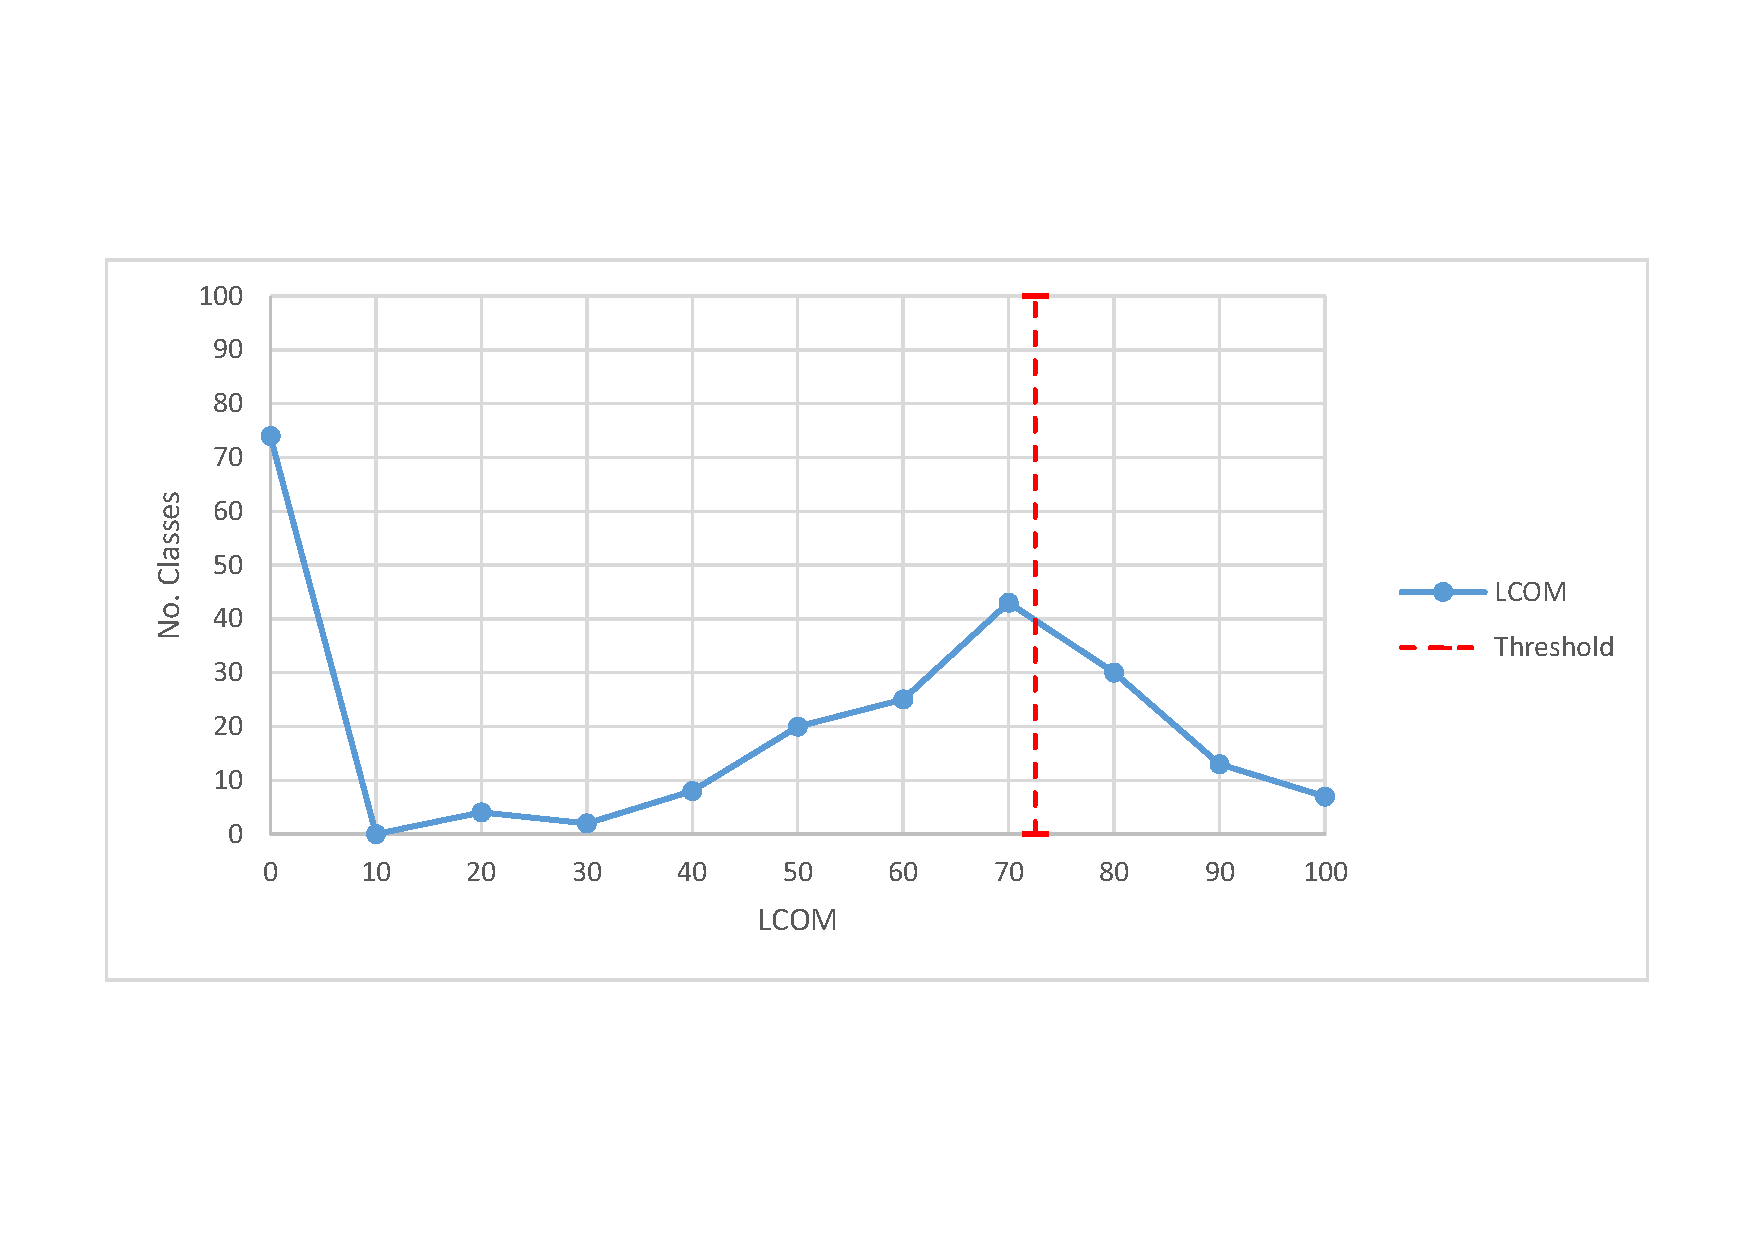
\includegraphics[width=\textwidth]{images/threshold/lcom.pdf}
	\caption{Frequency chart of the LCOM metric}
	\label{fig:lcomdistribution}
\end{figure}



\textbf{CBO}: In general, higher values of CBO indicate fault prone classes. Our analysis show that 194 classes have a value of CBO less than 10, and that 4 classes have a value larger than 20. The maximum value of CBO is 30. This class is an example of a class that is hard to understand, harder to reuse, and more difficult to maintain. 


\begin{figure}
	\centering
	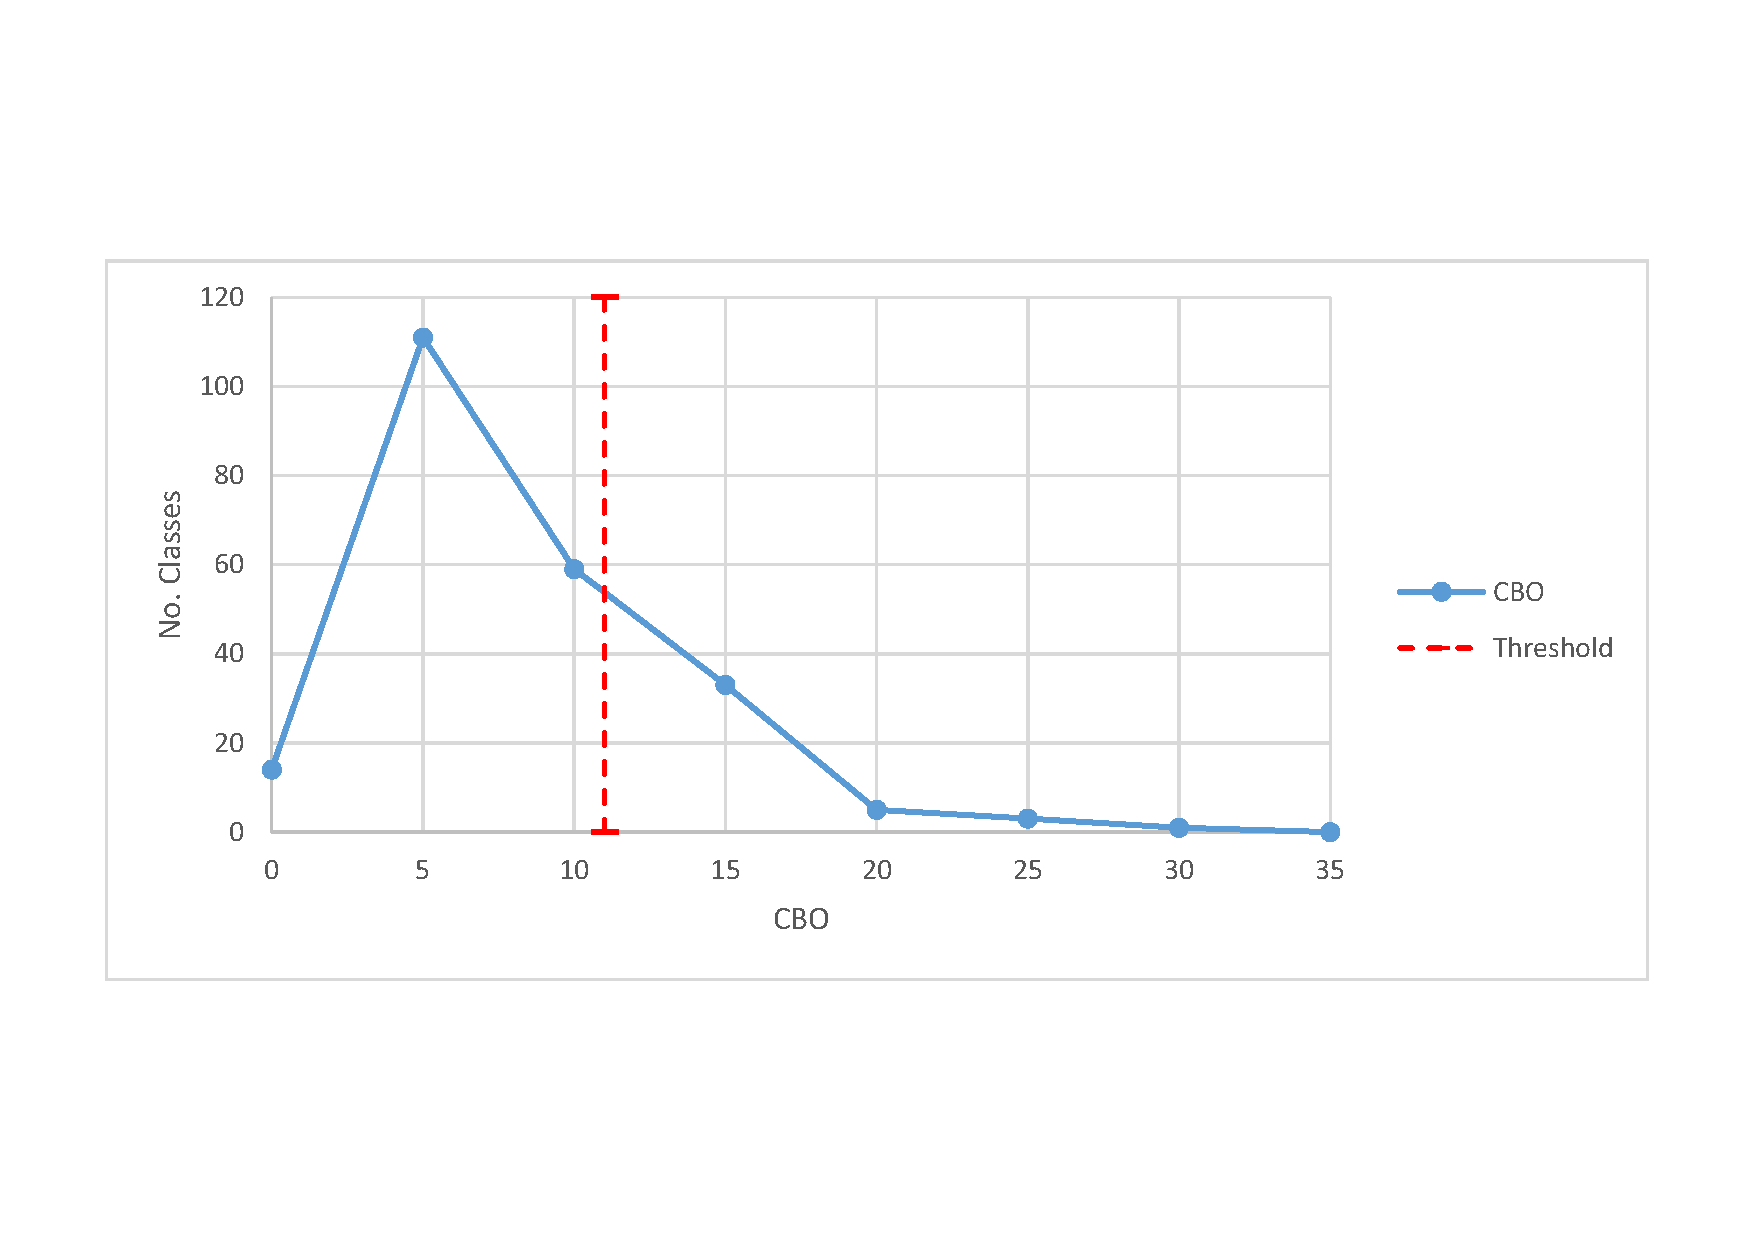
\includegraphics[width=\textwidth]{images/threshold/cbo.pdf}
	\caption{Frequency chart of the CBO metric}
	\label{fig:cbodistribution}
\end{figure}



\textbf{DIT}: DIT value appears to be generally low in the captured statistics. A class with DIT value of 0 is the root in a class hierarchy. Figure \ref{fig:ditdistribution} shows that 89 classes have a DIT value of 0, and 65 classes have a DIT value of 1. The median value suggests that most classes tend to be close to the root in the inheritance hierarachy. DIT metric can be used to determine whether the design is top heavy or bottom heavy\cite{chidamber1994metrics}. A design is top heavy if there are too many classes near the root, and bottom heavy if most classes are near the bottom of the hierarchy. The system appears to be top heavy by observing the empirical data of DIT, which indicates that there may be lack of reuse through inheritance. Classes with a DIT value of 2 and 3 indicates higher degree of reuse through inheritance. Widentified 70 classes in total with DIT value of 2 and 3. The maximum value of DIT is 4. These values show that inheritance is used in most of the classes to an optimal level. However, there may be some possibilities for improvements for classes with DIT value of 0. 

\begin{figure}
	\centering
	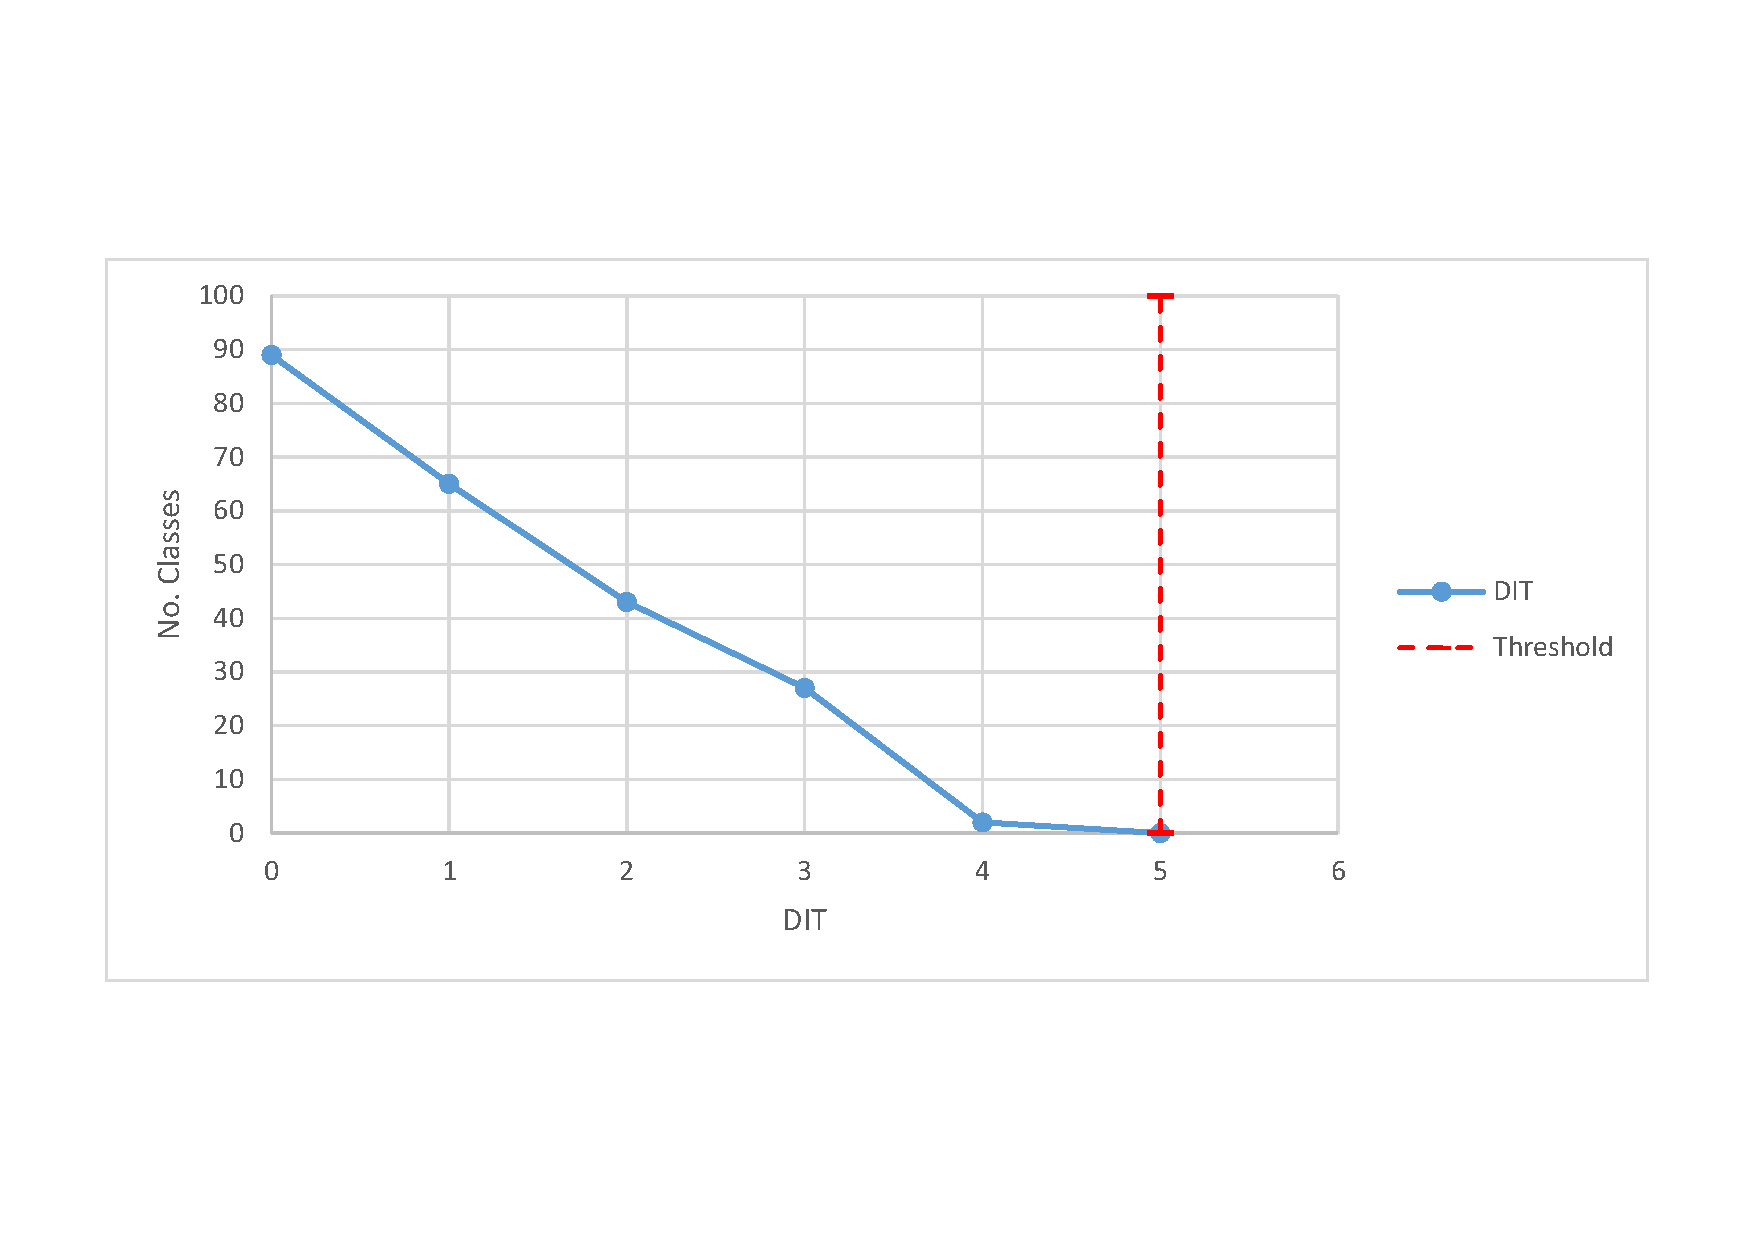
\includegraphics[width=\textwidth]{images/threshold/dit.pdf}
	\caption{Frequency chart of the DIT metric}
	\label{fig:ditdistribution}
\end{figure}


\textbf{NOC}: NOC metric measures the number of subclasses of a class. The median value of NOC show that most half of the classes has no immediate children, which indicates that inheritance may not be used enough. According to the Figure \ref{fig:nocdistribution}, approximately 86\% of the classes seem to have no subclasses, hence affecting the normal distribution due to a high value of kurtosis. In addition, the skewness value indicate that long tail is on the positive side of the peak (i.e., on the right side). Furthermore, the max value of NOC is 20, which may indicate a misuse of subclassing. Classes with high NOC value are difficult to modify, and they usually require more testing because of the effects on changes on all the children. 

\begin{figure}
	\centering
	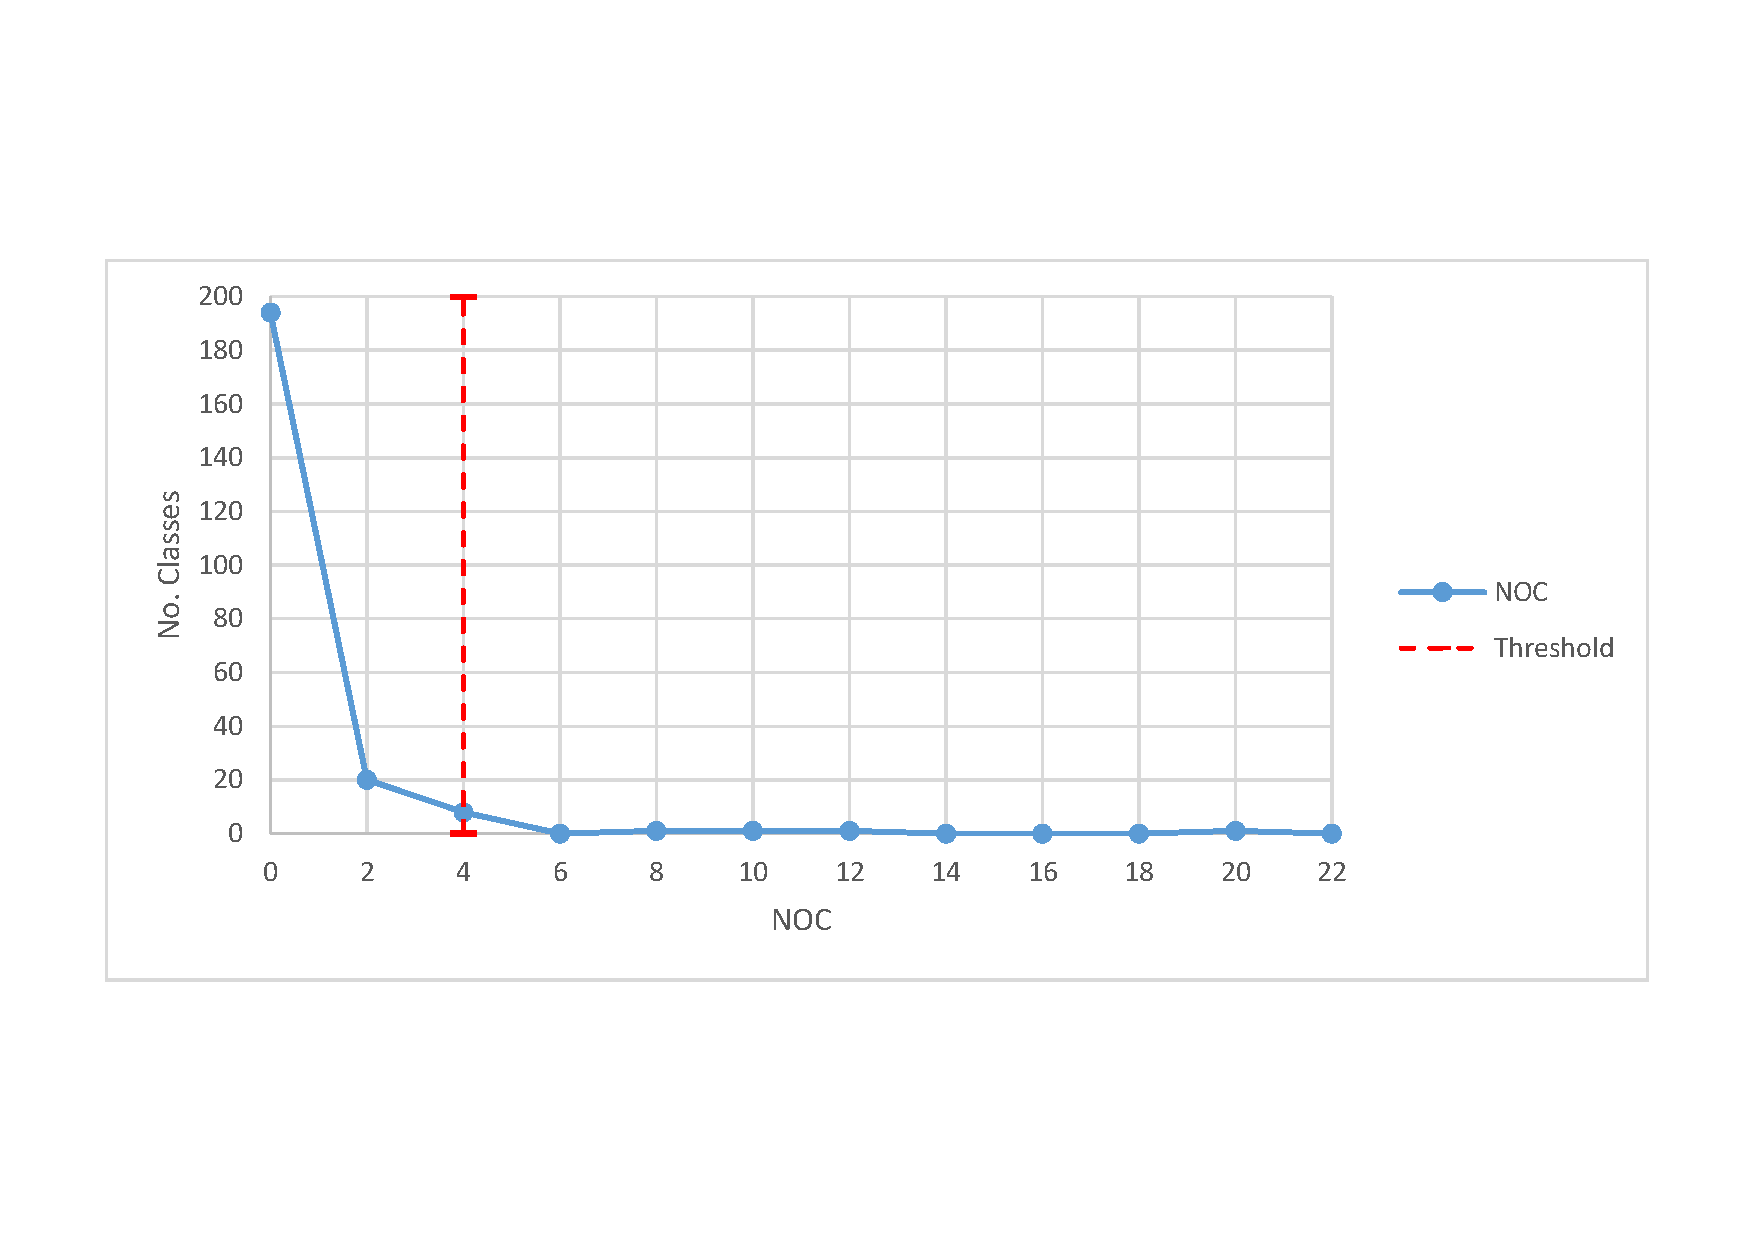
\includegraphics[width=\textwidth]{images/threshold/noc.pdf}
	\caption{Frequency chart of the NOC metric}
	\label{fig:nocdistribution}
\end{figure}


\textbf{RFC}: Classes with large RFC tend to be complex and have decreased understandability. Testing classes with large RFC is more complicated. The RFC statistics reveal that majority of the classes have a RFC of less than 20. There are only 22 classes with a value of RFC larger than 30, where 2 of them have a value larger than 100. The maximum value of RFC in this system is 115. A suggestion would be to inspect classes with higher values of RFC.

\begin{figure}
	\centering
	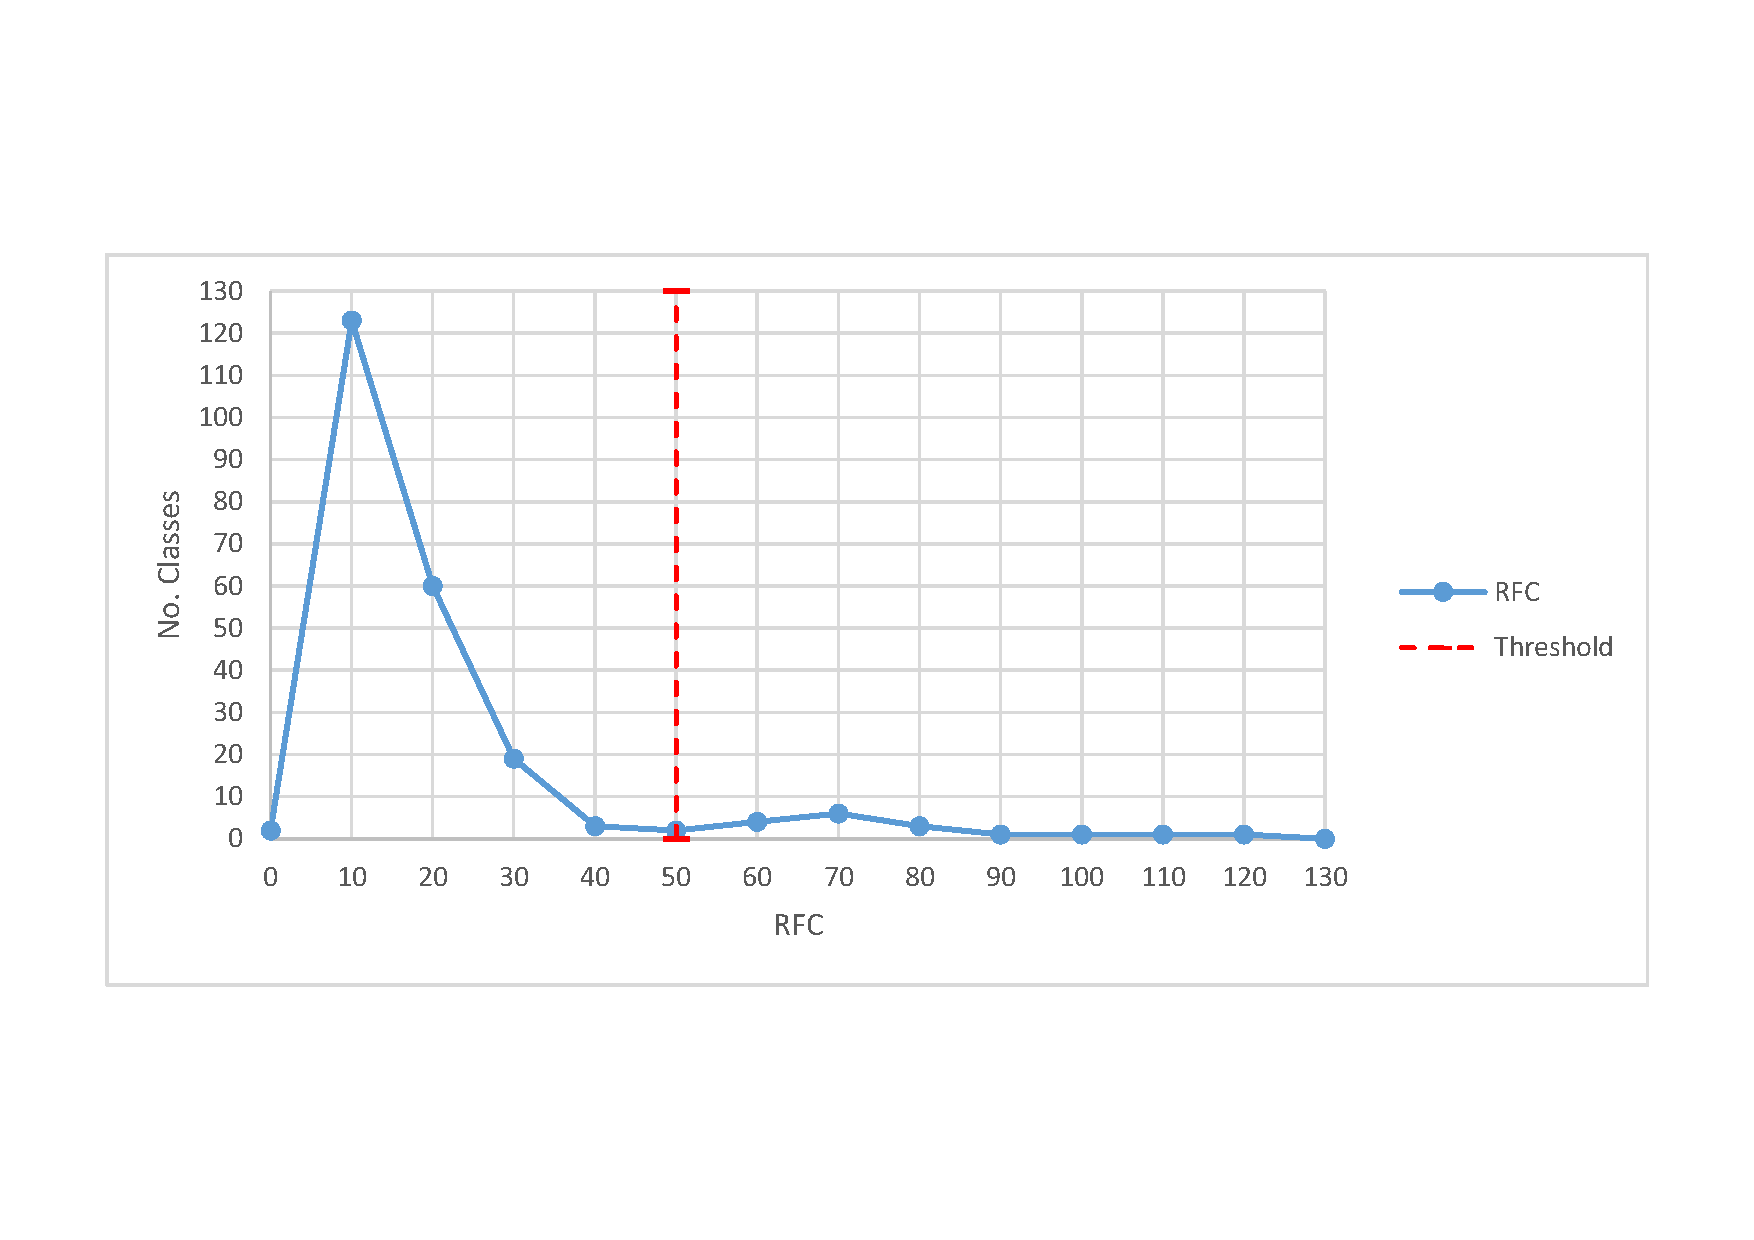
\includegraphics[width=\textwidth]{images/threshold/rfc.pdf}
	\caption{Frequency chart of the RFC metric}
	\label{fig:rfcdistribution}
\end{figure}

\textbf{WMC}: We observe that majority of the classes have a value of WMC less than 10 by examining Figure \ref{fig:wmcdistribution}. More precisely, 123 classes has a value of WMC less than 10. Moreover, 5 classes have a value of WMC2 larger than 100. The maximum value of WMC is set to 325.

\begin{figure}
	\centering
	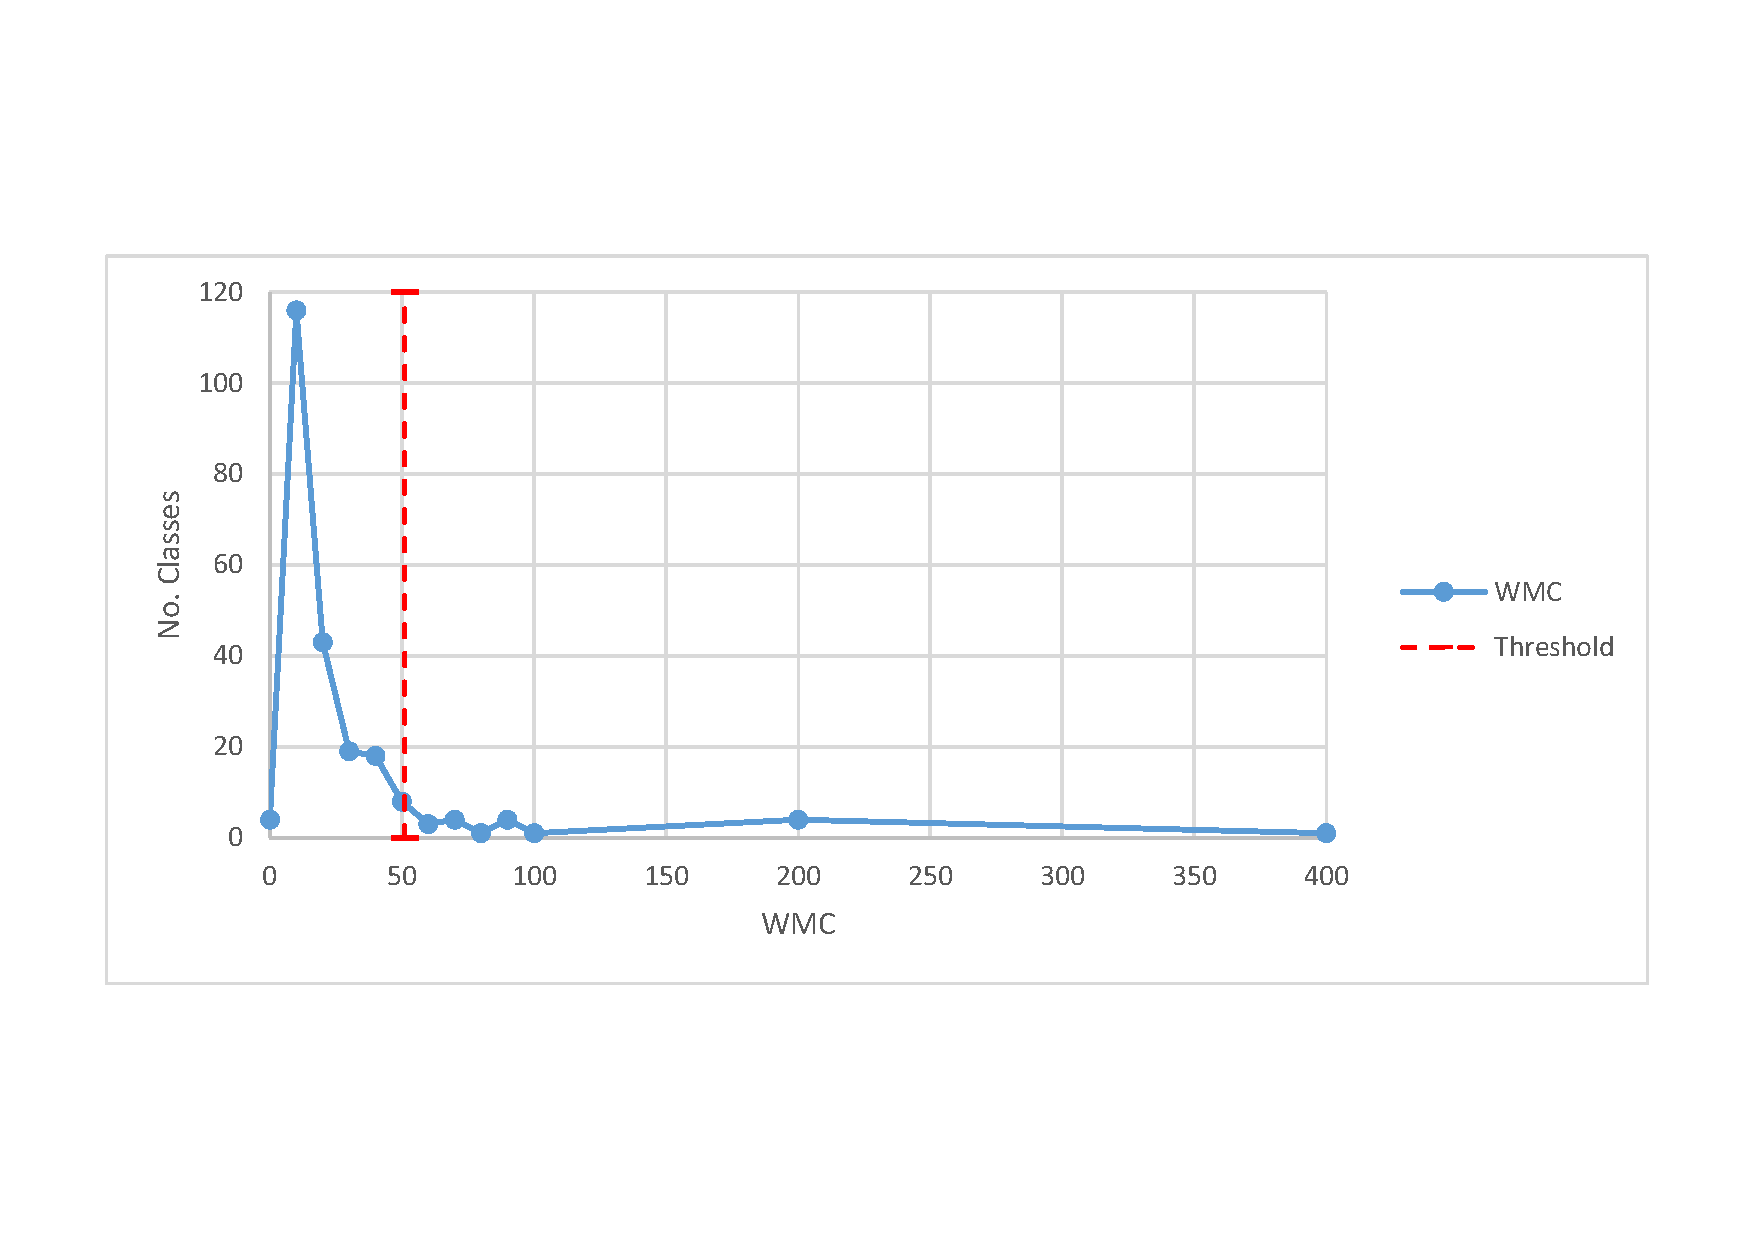
\includegraphics[width=\textwidth]{images/threshold/wmc.pdf}
	\caption{Frequency chart of the WMC metric}
	\label{fig:wmcdistribution}
\end{figure}

\textbf{NIM and NIV}: The NIM and NIV metrics report the number instance methods and instance variables in a class. Our analysis show that most classes are small. The sample mean of NIV tells us that each class has an average of 2 instance variables. The maximum value of NIV is 18, indicating that there is at least one class that contains 18 instance variables. The sample mean of NIM show us that each class has an average of 8 instance methods. More precisely, there are 170 classes with value of NIM less than 10. The maximum value of NIM is 48, which indicates that there is at least one class contains 48 methods. 


%\begin{figure}[!tbp]
%\centering
%\begin{subfigure}{\textwidth}
%	\centering
%	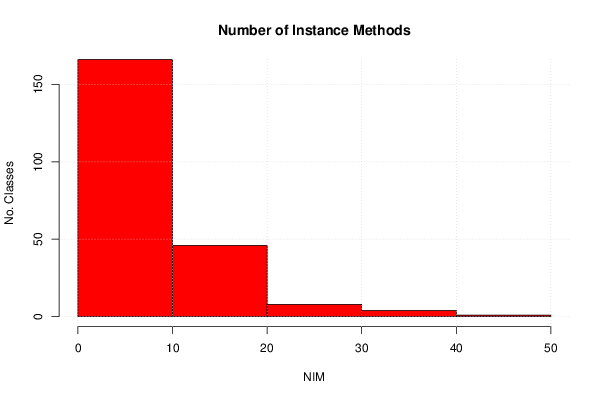
\includegraphics[width=.5\textwidth]{images/NIM.png}
%	\caption{Frequency chart of the NIM metric}
%	\label{fig:nimdistrubition}
%\end{subfigure}
%\begin{subfigure}{\textwidth}
%	\centering
%	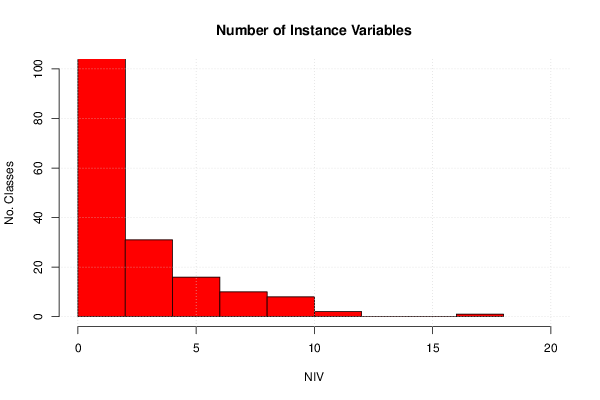
\includegraphics[width=.5\textwidth]{images/NIV.png}
%	\caption{Frequency chart of the NIV metric}
%	\label{fig:nivdistrubtion}
%\end{subfigure}
%\caption{Frequency chart of the NIM and NIV metric}
%\end{figure}


%Good refactoring would be to look at all the classes and see where we could use more abstraction. Reducing redundancy would reduce code size and speed. 

\subsection{Obect-Oritented Metrics for the Components}
\label{subsec:oometric-comp}
Descriptive statistics in Table \ref{tab:oometrics-firmus} reveal statistics for class level metrics for the whole project. However, the statistics do not say anything about class level metrics in the different components. Some of the components may have good OO-metric values, while other components have bad statistics. To identify components that are more fault-prone, we calculated descriptive statistics for each component.

\subsubsection{Component A}
Component A contains 53 files. Among these files, we identified 37 classes and 5427 lines of code. Figure \ref{fig:algraph} presents the frequency distribution of the measured OO-metrics. Table \ref{tab:oometrics-al} presents common descriptive statistics of the metric distribution.

\begin{table}[]
\resizebox{\textwidth}{!}{
\centering
\caption{OO-metrics and descriptive statistics for Component A}
\label{tab:oometrics-al}
\begin{tabular}{|l|l|l|l|l|l|l|l|}
\hline
\textbf{Metric} & \textbf{Min} & \textbf{Max} & \textbf{Median} & \textbf{Sample Mean} & \textbf{Standard Deviation} & \textbf{Kurtosis} & \textbf{Skewness} \\ \hline
LCOM            & 0            & 94           & 62              & 46.405               & 34.321      & -1.477  & -0.472               \\ \hline
DIT             & 0            & 4            & 2               & 1.567                & 1.167               &  -0.707 & 0.270      \\ \hline
CBO             & 0            & 30           & 6               & 6.758                & 6.639             &  4.00 & 1.766       \\ \hline
NOC             & 0            & 8            & 0               & 0.758                & 1.706             &    8.508 & 2.743      \\ \hline
RFC             & 6            & 115          & 38            & 43.649               & 31.515               &      -0.708 & 0.559 \\ \hline
NIM             & 4            & 40           & 10              & 13.135                 & 8.891               &    3.674 & 1.991    \\ \hline
NIV             & 0            & 12           & 1               & 2.270                  & 2.969              &  3.694 & 1.917       \\ \hline
WMC           & 3            & 194          & 19              & 31.081                 & 36.554              &    10.362 & 2.821    \\ \hline
\end{tabular}}
\end{table}

The DIT values indicate that inheritance hierarchies is somehow flat. Classes with flat inheritance hierarchy usually hints that reuse through inheritance is not used. There are 8 classes with flat inheritance hierarchy. Rest of the classes inherit for at least one class. The max value captured show that some classes have deep hierarchy. Higher values for DIT indicates higher degree of reuse, but as trade off, it may potentially increase the complexity of the class. Moreover, the results indicate that most classes only have a few subclasses. We identified 29 classes with no children. Moreover, we idenfied a class with a NOC value of 8. 

The results show that 32.4\% (i.e., 12 classes) of all classes in Component A are strongly cohesive, which implies that more than half of the classes show lack of cohesion. We notice that two classes has LCOM values larger than 90 by examining Figure \ref{fig:algraph}. These classes indicate loose class structures. The kurtosis value of LCOM is negative, so we can consider LCOM having a flat distribution, which can be seen Figure \ref{fig:algraph}. 

Most classes have small CBO values, indicating that they are self-contained. However, the frequency distribution shows that few of the classes are strongly coupled. There is one class in component B with a CBO value of 29. This class may potentially be fault-prone class. Additionally, this class may affect its reusability and maintainability. This particular class has LCOM value of 62, WMC value of 95, and RFC value of 25, hence being a possible Large Class code smell.

The results show that each class have at least two methods. More than half of the classes have low RFC values, which indicates greater polymorphism. However, there are few classes in this component that has larger values of RFC. The maximum RFC value is 115, and classes with high RFC are usually difficult to maintain and test. 

The values of WMC rangs from 3 to 194. The median value indicate that at least 50\% of the classes have a cyclomatic complexity of 17 or less. However, the sample mean is revealed to be larger than the median value. This implies that there are few classes with large values of WMC, which is evident by inspecting the standard deviation value.

There are few classes with large values of NIV. At least 50\% of the classes have one instance variable or less. The largest number of instance variables in a class is 12. This may potentially imply that the system does not apply information hiding principle appropriately for this class. The same class have its LCOM value at 90, which indicates that most variables are not shared across the member functions. Furthermore, each class is revealed to have at least four instance methods. At least 50\% of the classes have 10 instance methods or less. This means that rest of the classes have more than 10 instance methods, which indicates that classes may potentially provide several services to other classes. This could be the reason behind large values of LCOM. The maximum value of NIM captured is 40. There are two classes with NIM value of 40, one having a WMC value of 194 and the other having a WMC value of 72. Both classes have a LCOM value larger than 90. This class may potentially be a \textit{Large Class}.


%AL: LogicsEngine
%Autrologic: LogicsUnitDetectionZone
%Autrologic: Logicsunit
%AL: LogicsUnitFad (kasnkje)
%BLC: AclibTranslator


\begin{landscape}
\setlength\LTleft{-.5in}
	\begin{figure}
	\centering
	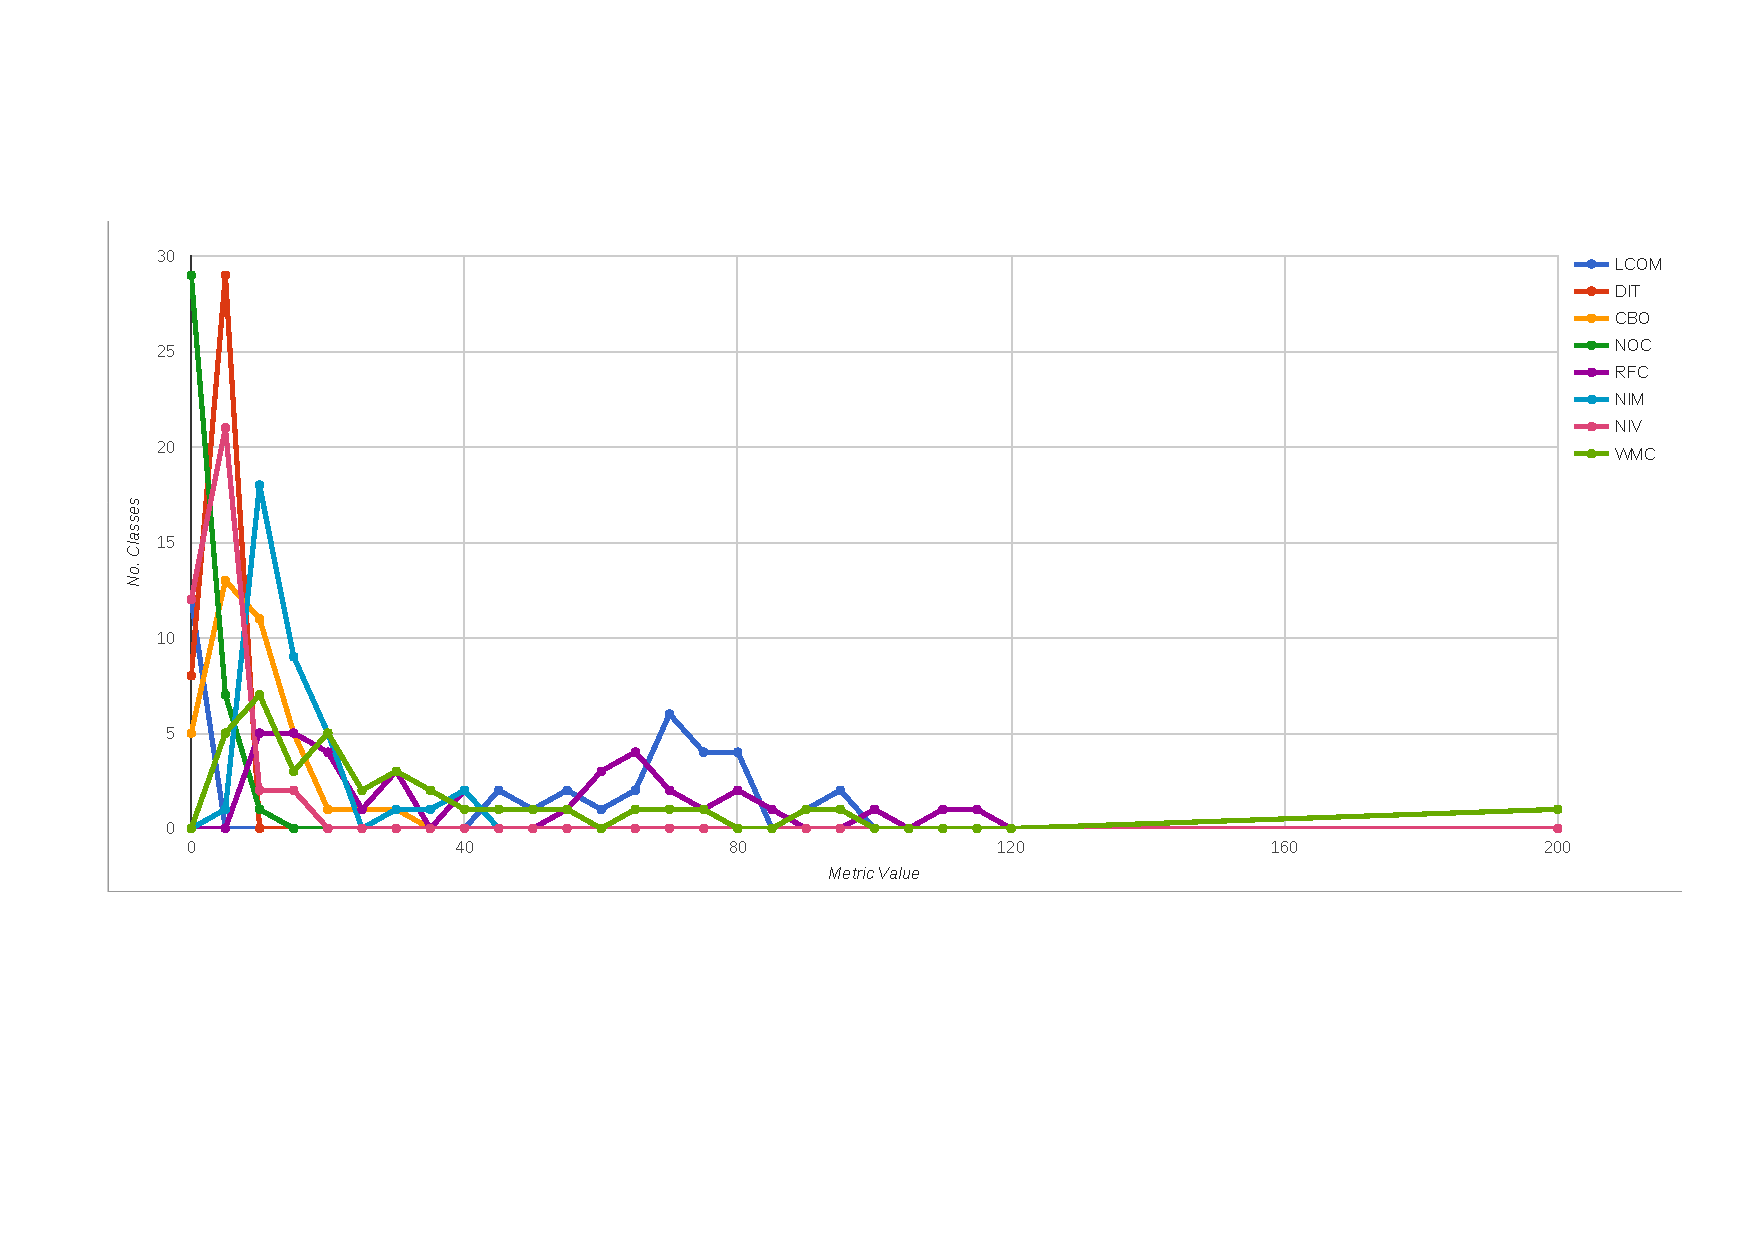
\includegraphics[width=\textwidth]{images/pdf/al.pdf}
	\caption{Frequency distribution of OO-metrics in Component A}
	\label{fig:algraph}
	\end{figure}
\end{landscape}

% 2 large code smell


\subsubsection{Component B}
We identified 23 classes in Component B. These classes are spread across 42 files, which in total contains 3905 lines of code. Figure \ref{fig:blcgraph} presents a frequency chart of the OO-metric results for Component B. Table \ref{tab:oometrics-blc} presents descriptive statistics of the analyzed metrics.

The values of LCOM in Component B range from 22 to 91, which indicates that none of the classes in Component B are strongly cohesive. There are only two classes with LCOM values below 50, both having low values in terms of complexity, method count, coupled objects, and instance variables. The WMC metric values range from 3 to 325. We decided to examine the class with max value of WMC. This class has a LCOM value of 74, and a CBO value of 10. Its RFC value is 44, while NIM is 36. This class has no subclasses, but it does inherit methods and variables from one superclass. This class is revealed to be the most complex class in the system in terms of cyclomatic complexity. Moreover, there are 8 classes in this component with a LCOM value of 66. We did notice that 4 of these classes has identical DIT, CBO, RFC, NIM, NIV, and WMC values by examining the metrics of the metrics for these classes. Manual inspection of the classes did not reveal any duplicated code. In terms of refactoring, we do think that all these classes need the same effort.

% to mulige store klasser.


\begin{table}[]
\resizebox{\textwidth}{!}{
\centering
\caption{OO-metrics and descriptive statistics for Component B}
\label{tab:oometrics-blc}
\begin{tabular}{|l|l|l|l|l|l|l|l|}
\hline
\textbf{Metric} & \textbf{Min} & \textbf{Max} & \textbf{Median} & \textbf{Sample Mean} & \textbf{Standard Deviation} & \textbf{Kurtosis} & \textbf{Skewness} \\ \hline
LCOM            & 22           & 91          & 66              & 63.348               & 15.916   & 1.179  & -0.761                   \\ \hline
DIT             & 0           & 1           & 1             & 0.609              & 0.499        & -1.950  & -0.477                 \\ \hline
CBO             & 1          & 21           & 5              & 6.13                & 4.799       & 2.653  & 1.350                  \\ \hline
NOC             & 0            & 1           & 0               & 0.087                & 0.288  & 8.605  & 3.140                       \\ \hline
RFC             & 6            & 48          & 9              & 14.217              & 11.977    & 2.867  & 1.831                    \\ \hline
NIM             & 6           & 48           & 9               & 13.434                & 10.974   & 3.822  & 1.986                      \\ \hline
NIV             & 1            & 10           & 2               & 3                & 2.504       &  2.51 & 1.711                  \\ \hline
WMC            & 3            & 325          & 19              & 35.826               & 66.796   & 17.288  & 3.964                     \\ \hline
\end{tabular}}
\end{table}


\begin{landscape}
\setlength\LTleft{-.5in}
	\begin{figure}
	\centering
	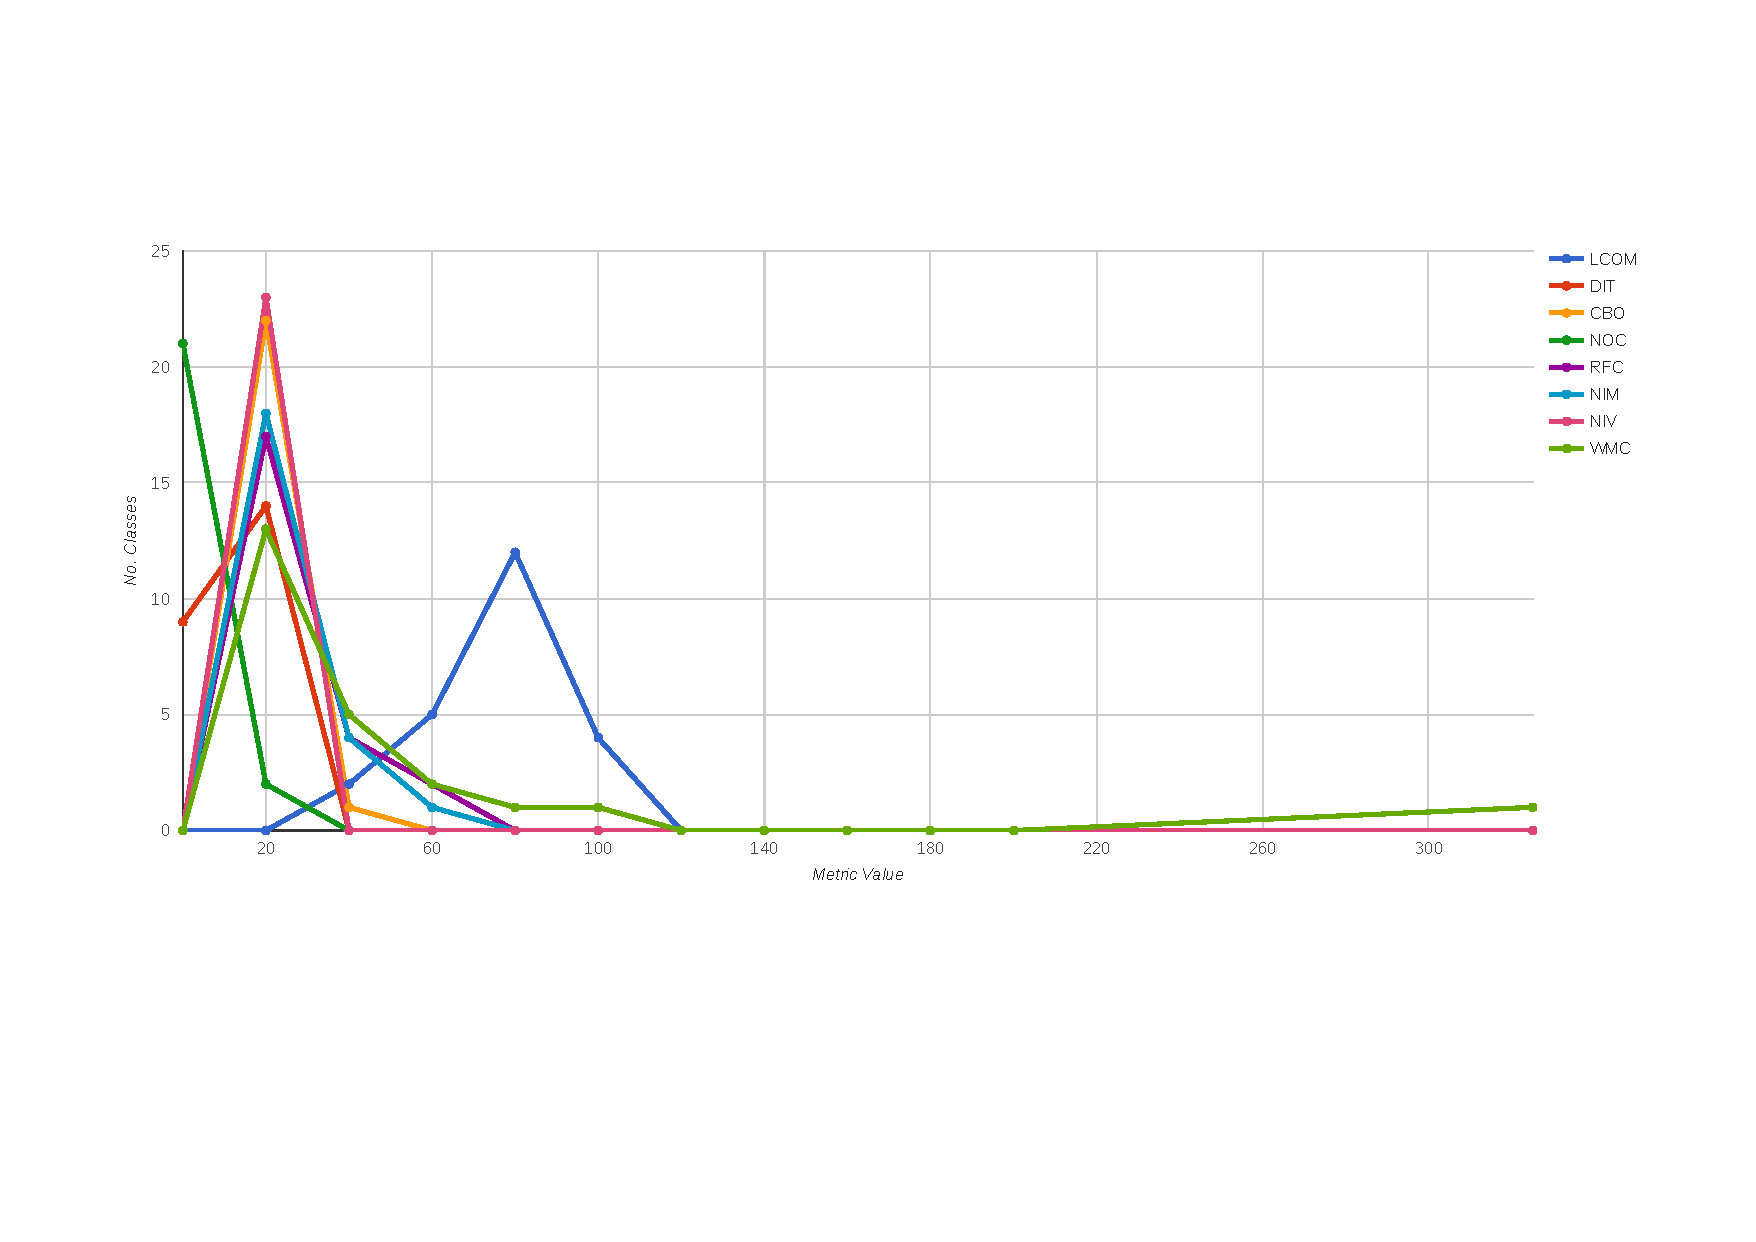
\includegraphics[width=\textwidth]{images/pdf/blc.pdf}
	\caption{Frequency distribution of OO-metrics in Component B}
	\label{fig:blcgraph}
	\end{figure}
\end{landscape}



\subsubsection{Component C}
Our analysis shows that component C contains 29 files, 20 classes, and 4792 lines of code. We present the descriptive statistics for component C in Table \ref{tab:oometrics-config}, and the frequency distribution of the metrics in Figure \ref{fig:confgraph}.

LCOM values of Component C range from 0 to 89. The median value reveal that more than half of the classes have LCOM value of 60 or more, indicating possibilities for design improvements by splitting up the classes. DIT and NOC metric values is very low, implying that inheritance may potentially not be used enough. Moreover, CBO values range from 1 to 19. Each class has a CBO value of 5 in average. One of the classes have a CBO value of 19. This class prevents reuse due to its modular design. Strong coupling complicates a system since a class is harder to understand and modify. The WMC metric values range from 3 to 106. The median value suggests that complexity in this component is well managed for most classes. However, we identified one class with a WMC value of 106. This particular class has a LCOM value of 63, and is coupled to 18 other objects. RFC, and NIM values of this class is set to 26, which are the maximum values that we analyzed for the corresponding metrics. All these values are an indication of a possible fault-prone and complex class. In addition, this class may potentially be affected by the Large Class code smell.

% 1 large class code smell, mulig 2. 



\begin{table}[]
\resizebox{\textwidth}{!}{
\centering
\caption{OO-metrics and descriptive statistics for Component C}
\label{tab:oometrics-config}
\begin{tabular}{|l|l|l|l|l|l|l|l|}
\hline
\textbf{Metric} & \textbf{Min} & \textbf{Max} & \textbf{Median} & \textbf{Sample Mean} & \textbf{Standard Deviation} & \textbf{Kurtosis} & \textbf{Skewness} \\ \hline
LCOM            & 0            & 89           & 61              & 54.8                 & 22.139    & 1.015  & -1.089                     \\ \hline
DIT             & 0            & 1            & 0               & 0.1                  & 0.308  & 7.037  & 2.888                       \\ \hline
CBO             & 1            & 19           & 4.5               & 6.5                 & 5.587     & -0.045  & 1.030                    \\ \hline
NOC             & 0            & 1            & 0               & 0.05                    & 0.223     & 20  & 4.472                        \\ \hline
RFC             & 3            & 26           & 8.5             & 10.3                 & 5.741   & 1.825 & 1.363                      \\ \hline
NIM             & 3            & 26           & 8.5             & 9.85                 & 5.153    & 3.967  & 1.626                     \\ \hline
NIV             & 0            & 9            & 2               & 3.15                 & 3.013   & -0.217  & 1.084                      \\ \hline
WMC           & 3            & 106          & 12.5              & 27.65                 & 30.975   & 1.472  & 1.544                     \\ \hline
\end{tabular}}
\end{table}



\begin{landscape}
\setlength\LTleft{-.5in}
	\begin{figure}
	\centering
	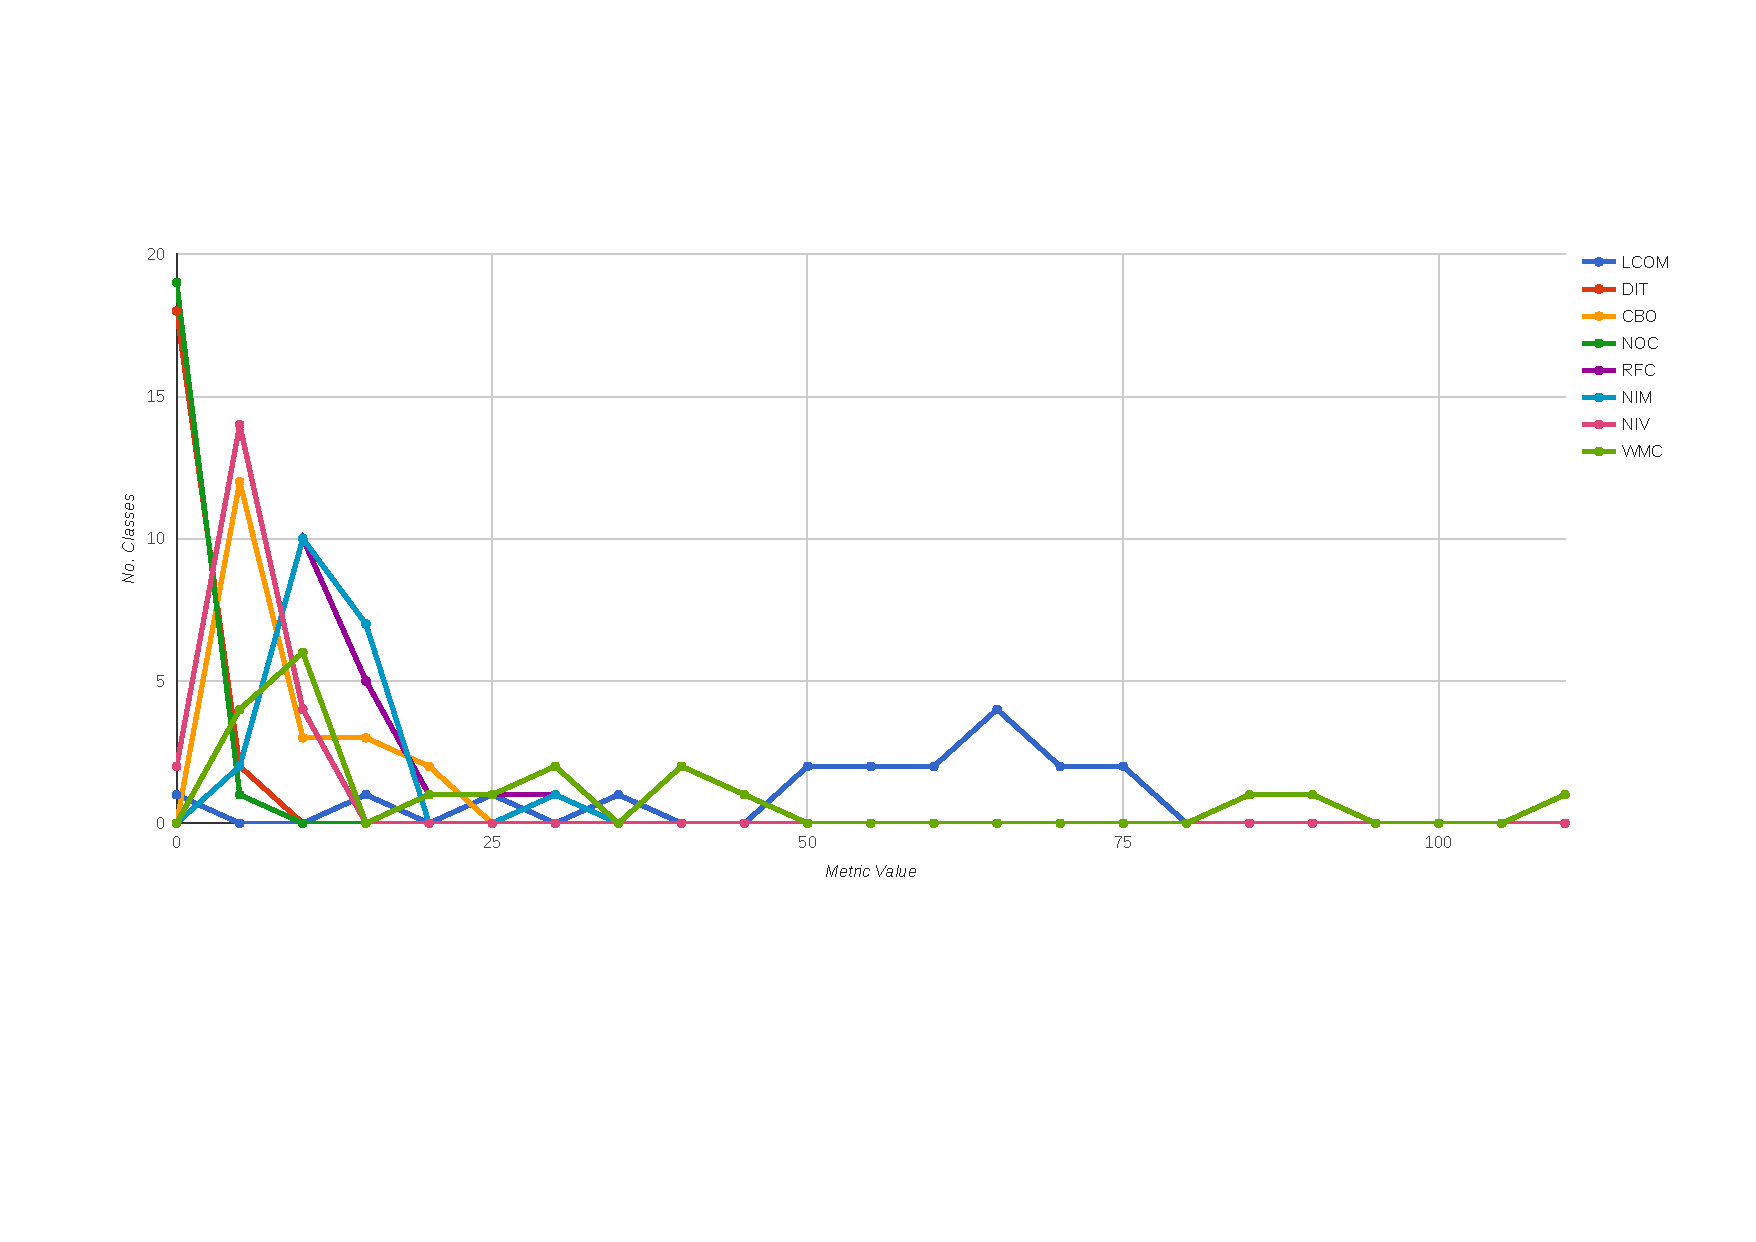
\includegraphics[width=\textwidth]{images/pdf/conf.pdf}
	\caption{Frequency distribution of OO-metrics in Component C}
	\label{fig:confgraph}
	\end{figure}
\end{landscape}


\subsubsection{Component D}
Our analysis show that Component D consists of 13 files and 1647 lines of code. Among these files, we were only able to identify one class. This class has LCOM value of 68. Furthermore, our results show a DIT value of 1 for this class, and a NOC value of 0. The CBO value is set to 10. The values of RFC, and NIM have a value of 8. Moreover, the class has one instance variable. The sum of complexity in this class is 17.

\subsubsection{Component En}
Similar to Component D, our analysis identified only one class among 3 files and 367 lines of code in Component En. The metrics are very similar to Component D metrics. The class has a LCOM value of 62, indicating that the class may potentially have low cohesion in some of the methods. However, compared to Component D, this class is only coupled to one object. The sum of complexity of methods in this class is 15.

\subsubsection{Component Ex}
Our analysis found 48 files in Component Ex. These files consist of 4089 lines of code, and among these, we identified 86 classes. 38\% of the number of classes of the system are located in this component. Table \ref{tab:oometrics-ex} presents the descriptive statistics for Component Ex, while Figure \ref{fig:exgraph} presents the frequency distribution of the measured metrics. 

Despite the fact that at least 50\% of the classes have high cohesion, there are still many classes that show lack of cohesion. Our results show that there are 22 classes with LCOM value larger than 50, whereas 6 classes have a LCOM value of 80 or more. There are 2 classes with LCOM value of 100. Moreover, the average cyclomatic complexity of the classes have a value of 8.744, while the median has a value of 7. These values imply that most classes may have more polymorphism and less complexity. Figure \ref{fig:exgraph} shows that there are only one 8 classes with value of WMC larger than 20, whereas the maximum value is 41. These values indicate that the complexity is well managed to this point. We observe that only 7 classes are self-contained by examining the CBO values. Rest of the classes are coupled to other objects. The majority of the classes has a CBO value of 5 or less. There is only one class with CBO value of 16, indicating that this class may potentially be difficult to understand and maintain. 

\begin{table}[]
\resizebox{\textwidth}{!}{
\centering
\caption{OO-metrics and descriptive statistics for Component Ex}
\label{tab:oometrics-ex}
\begin{tabular}{|l|l|l|l|l|l|l|l|}
\hline
\textbf{Metric} & \textbf{Min} & \textbf{Max} & \textbf{Median} & \textbf{Sample Mean} & \textbf{Standard Deviation} & \textbf{Kurtosis} & \textbf{Skewness} \\ \hline
LCOM            & 0           & 100          & 0               & 26.302               & 33.082    & -0.971 & 0.756                    \\ \hline
DIT             & 0            & 3            & 2               & 1.581                & 1.121   & -1.313   & -0.234                     \\ \hline
CBO             & 0            & 16           & 4               & 5.314                & 4.459  & -0.511   & 0.783                      \\ \hline
NOC             & 0            & 20           & 0               & 0.744                & 2.736    & 32.072   & 5.338                     \\ \hline
RFC             & 0            & 28           & 8               & 10.279               & 6.030    & 0.800  & 0.87                     \\ \hline
NIM             & 0            & 22           & 3               & 4.907                & 3.846   & 4.082  & 1.785                      \\ \hline
NIV             & 0            & 10           & 0               & 1.209                & 2.098  & 5.887  & 2.415                       \\ \hline
WMC            & 0            & 41          & 7              & 8.744                 & 8.117     & 3.91  & 1.882                   \\ \hline
\end{tabular}}
\end{table}


\begin{landscape}
\setlength\LTleft{-.5in}
	\begin{figure}
	\centering
	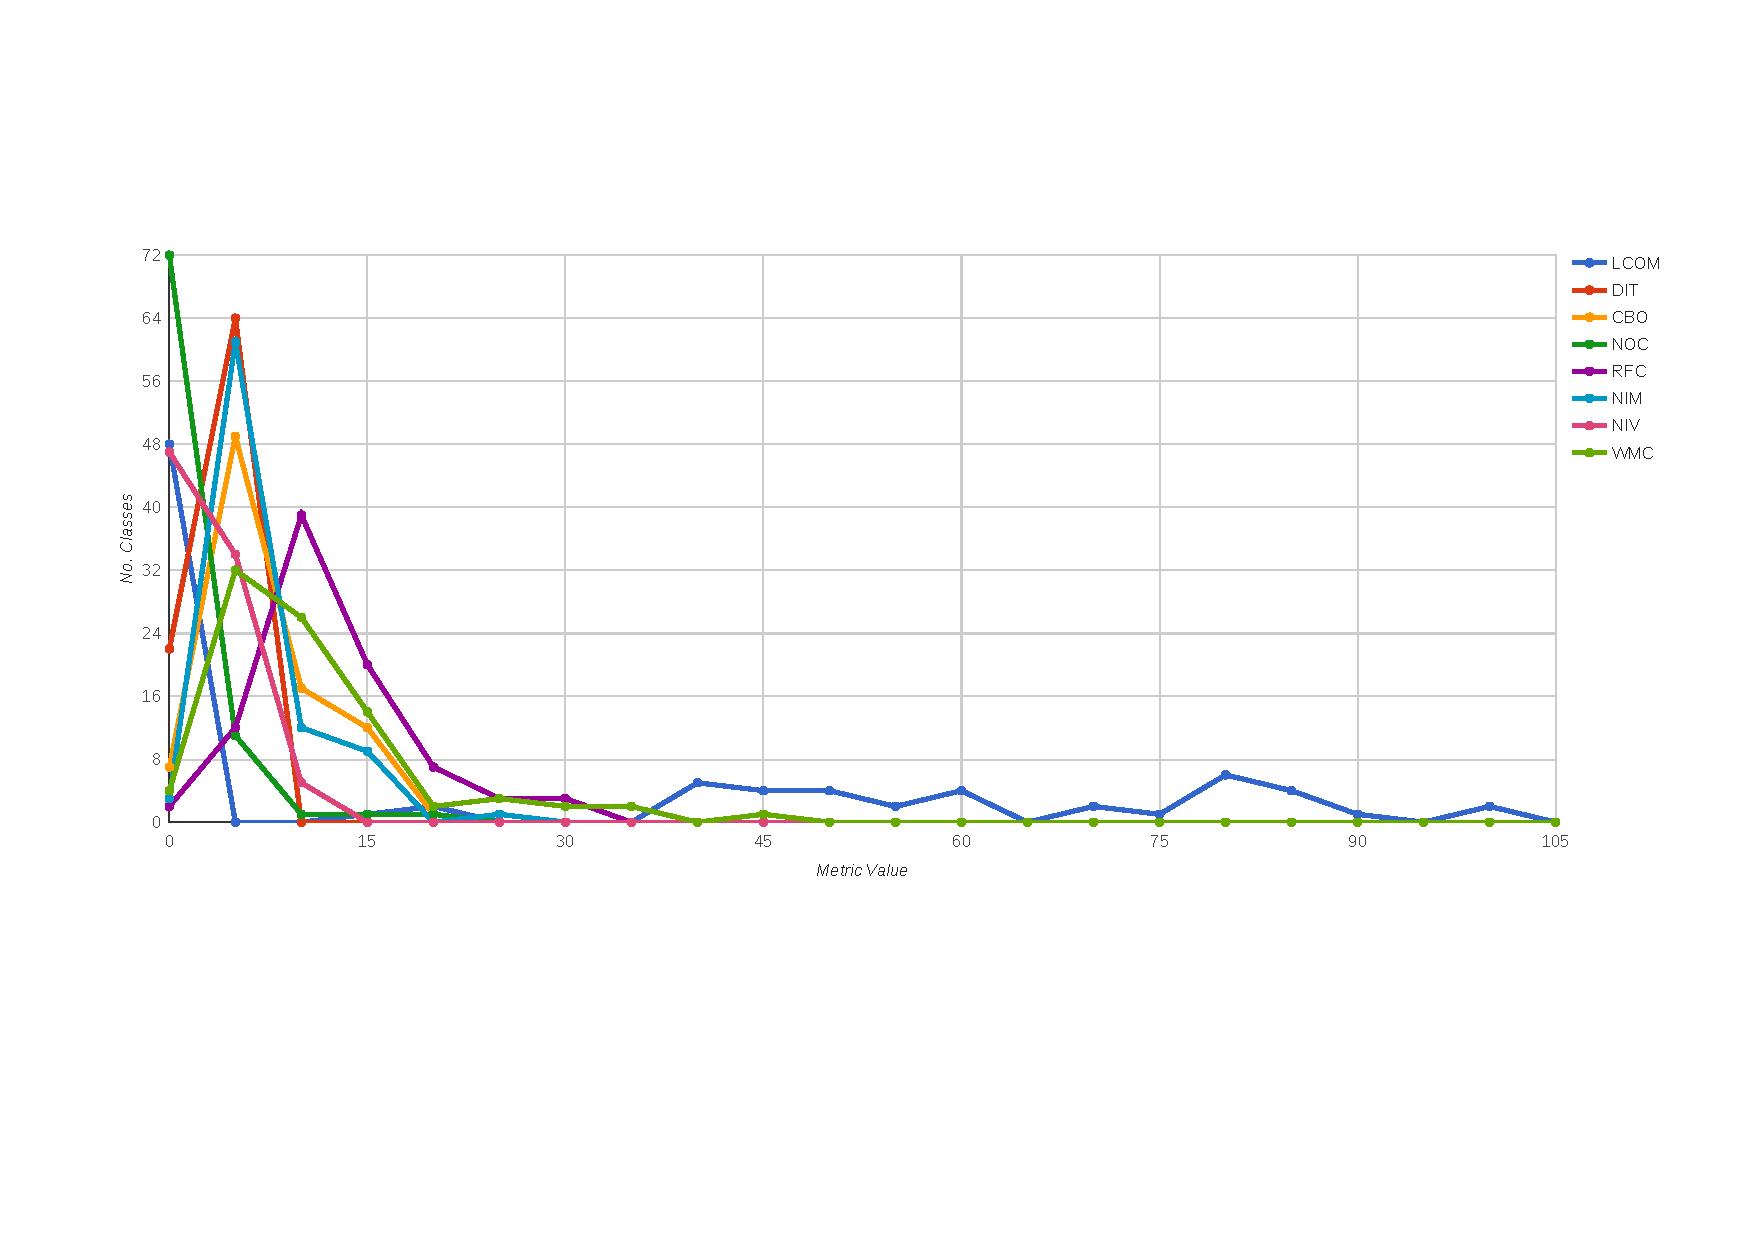
\includegraphics[width=\textwidth]{images/pdf/ex.pdf}
	\caption{Frequency distribution of OO-metrics in Component Ex}
	\label{fig:exgraph}
	\end{figure}
\end{landscape}


% GOd class detection: High WMC, low cohesion, number of attributes bigger than 20




\subsubsection{Component G}
Component G consists of 59 files. These files include 3701 lines of code and 32 classes. Descriptive statistics for Component G are summarized in Table \ref{tab:oometrics-guri}, and its frequency distribution of metrics are presented in Figure \ref{fig:gurigraph}. 

Overall, the statistics indicate that there are some accumulated DD in this component. The values of LCOM range from 0 to 94, whereas 8 classes have a LCOM value of 0. However, values of LCOM for rest of the classes are larger than 50. Moreover, the statistics show that at least 16 classes have a DIT value of larger than 0, which indicates a higher degree of reuse. There are 5 classes with subclasses in this component. The WMC metric values in this component range from 1 to 123, where only class has a value of WMC larger than 100. We decided to examine the class with WMC value of 123. The metric of that class reveal a LCOM value of 92, CBO value of 22, RFC value of 30, NIM value of 9, and NIV value of 18. These values show that this class is probably influenced by the Large Class code smell, and is a candidate for inspection and possible refactoring.



\begin{table}[]
\resizebox{\textwidth}{!}{
\centering
\caption{OO-metrics and descriptive statistics for Component G}
\label{tab:oometrics-guri}
\begin{tabular}{|l|l|l|l|l|l|l|l|}
\hline
\textbf{Metric} & \textbf{Min} & \textbf{Max} & \textbf{Median} & \textbf{Sample Mean} & \textbf{Standard Deviation} & \textbf{Kurtosis} & \textbf{Skewness} \\ \hline
LCOM            & 0            & 94           & 60              & 50.25                & 31.236    & -0.767  & -0.794                    \\ \hline
DIT             & 0            & 2            & 1               & 0.625                & 0.609    & -0.582  & 0.399                    \\ \hline
CBO             & 0            & 23           & 5.5             & 6.312                & 4.987    & 1.898  & 1.152                    \\ \hline
NOC             & 0            & 2            & 0               & 0.25                 & 0.622   & 4.231  & 2.357                      \\ \hline
RFC             & 2            & 30           & 9               & 10.187               & 6.382   & 2.178  & 1.356                      \\ \hline
NIM             & 0            & 29           & 7               & 8.437        & 5.459              & 5.669  & 1.745   \\ \hline
NIV             & 0            & 18           & 2               & 3.062          & 3.926          & 5.983 & 2.225    \\ \hline
WMC            & 1            & 123          & 12              & 19.437           & 24.794        & 9.572  & 2.824               \\ \hline
\end{tabular}}
\end{table}

\begin{landscape}
\setlength\LTleft{-.5in}
	\begin{figure}
	\centering
	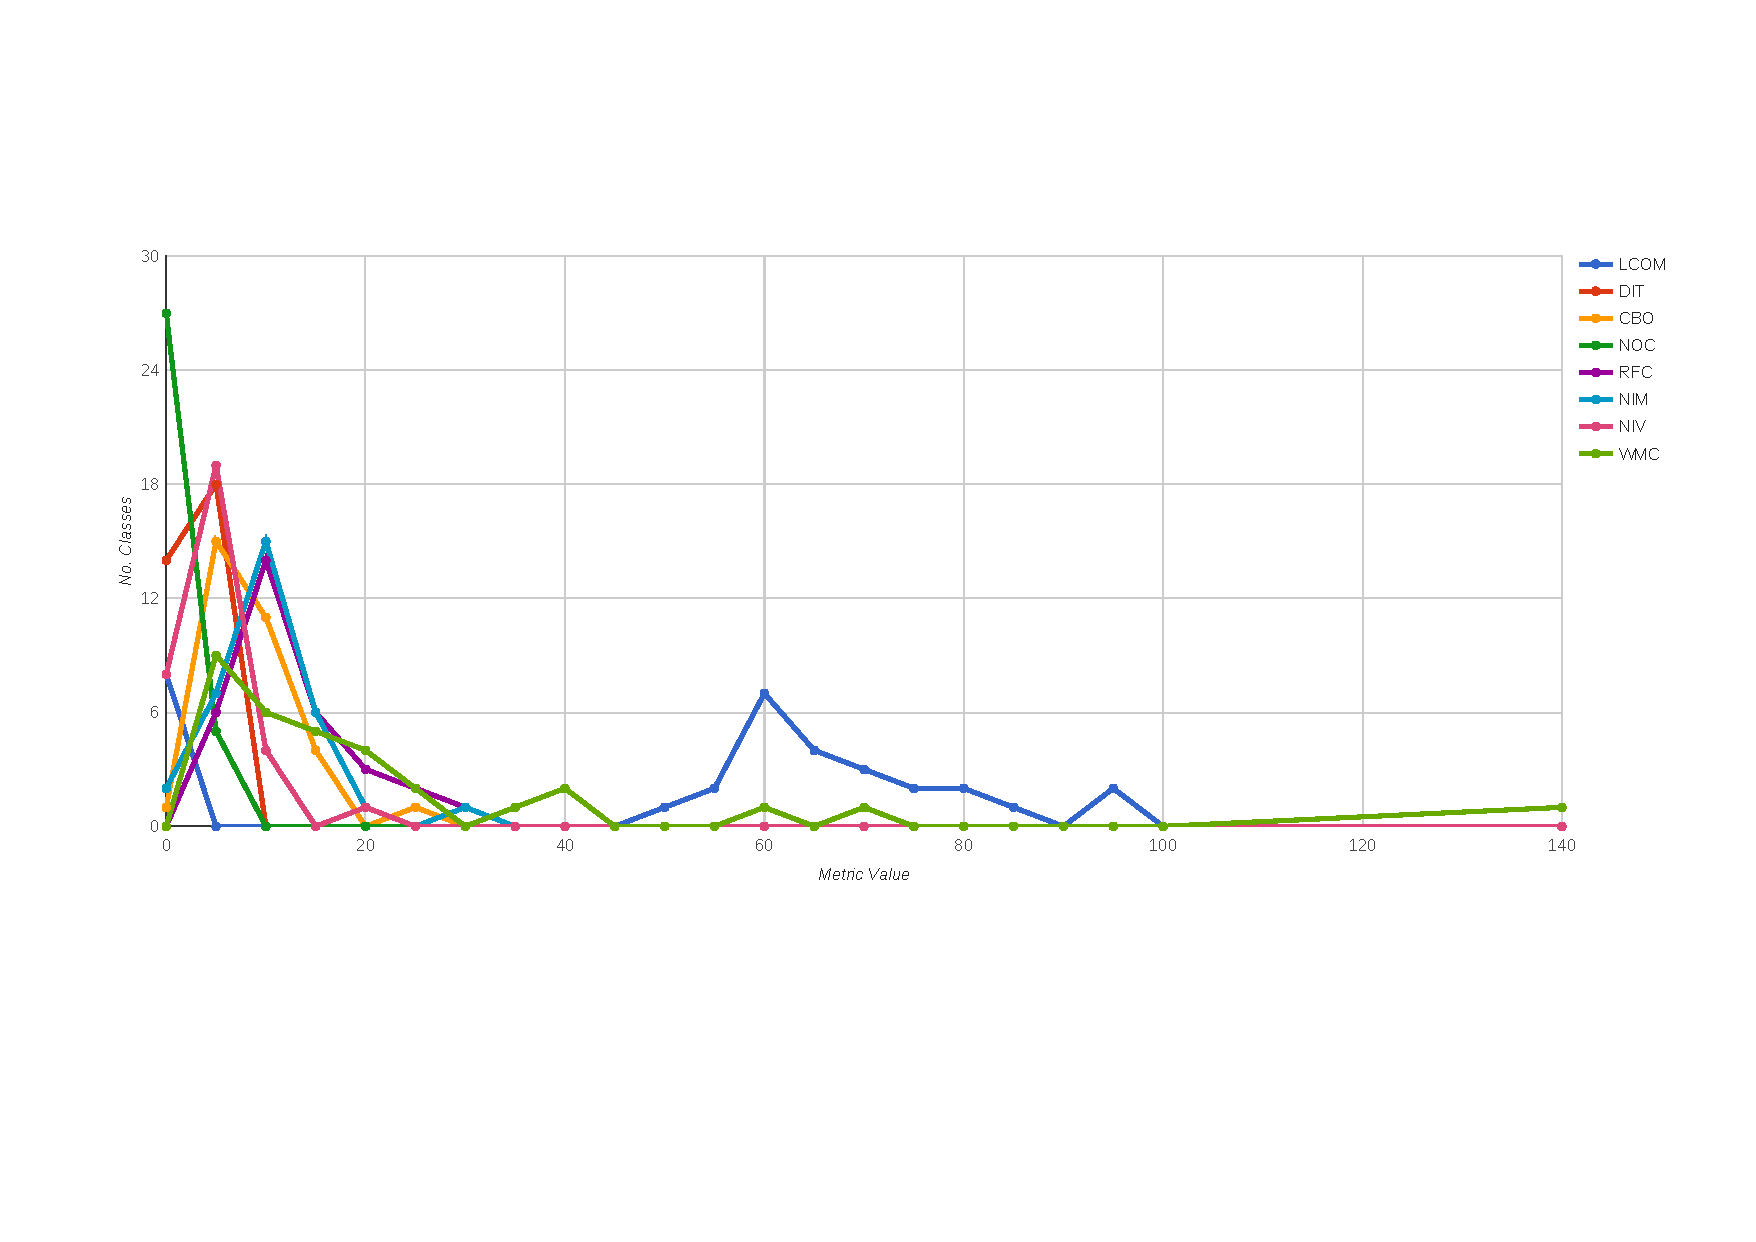
\includegraphics[width=\textwidth]{images/pdf/guri.pdf}
	\caption{Frequency distribution of OO-metrics in Component G}
	\label{fig:gurigraph}
	\end{figure}
\end{landscape}





\subsubsection{Component L}
Component L consists of 16 files, 849 lines of code. Among these, we identified 7 classes. Figure \ref{fig:loggraph} presents the frequency distribution of the metrics, while Table \ref{tab:oometrics-log} presents the descriptive statistics for this component. The values of LCOM range from 0 to 80. There are only 2 classes with LCOM value at 0. However, rest of the classes are showing lack of cohesion. These classes are candidates for inspection, and might eventually be split up into multiple classes. Moreover, 4 classes have a DIT value of 1. WMC metric values range from 4 to 42. There are only 2 classes with WMC values larger than 30.

\begin{table}[]
\resizebox{\textwidth}{!}{
\centering
\caption{OO-metrics and descriptive statistics for Component L}
\label{tab:oometrics-log}
\begin{tabular}{|l|l|l|l|l|l|l|l|}
\hline
\textbf{Metric} & \textbf{Min} & \textbf{Max} & \textbf{Median} & \textbf{Sample Mean} & \textbf{Standard Deviation} & \textbf{Kurtosis} & \textbf{Skewness} \\ \hline
LCOM            & 0            & 80           & 68              & 50.857               & 35.130  & -0.908  & -1.135                      \\ \hline
DIT             & 0            & 1            & 1               & 0.571                & 0.534    & -2.8  & -0.374                \\ \hline
CBO             & 1            & 14           & 6               & 6.714                & 4.609 & -0.712  & 0.327                         \\ \hline
NOC             & 0            & 0            & 0               & 0                    & 0     & N/A  & N/A                        \\ \hline
RFC             & 5            & 12           & 9               & 8.571                & 2.936    & -2.012  & -0.239                    \\ \hline
NIM             & 3            & 12           & 9               & 8.286         & 3.402            & -1.221  & -0.555            \\ \hline
NIV             & 0            & 5            & 1               & 1.571         & 2.070            & -0.535  & 1.120             \\ \hline
WMC            & 4            & 42          & 11              & 19.571                 & 14.524     & -1.521  & 0.577                   \\ \hline
\end{tabular}}
\end{table}



\begin{landscape}
\setlength\LTleft{-.5in}
	\begin{figure}
	\centering
	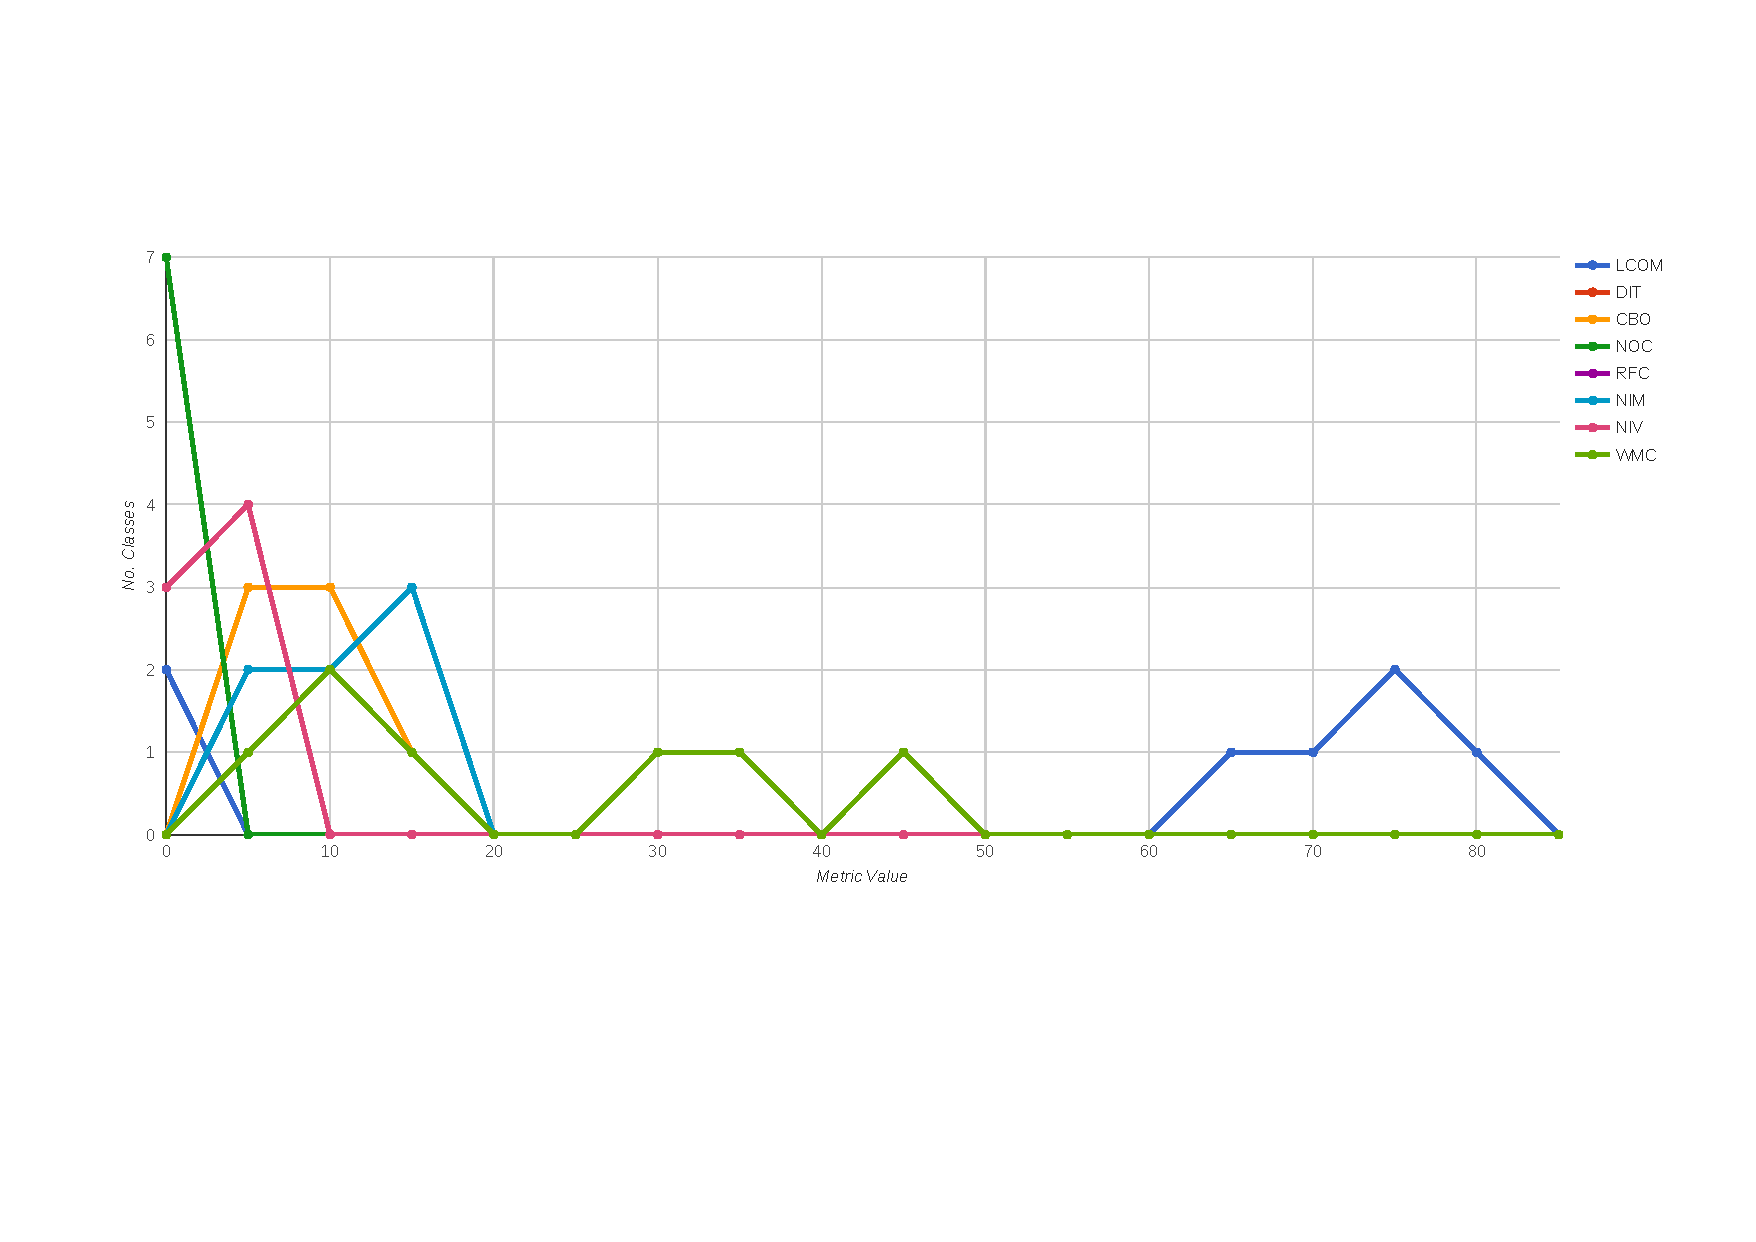
\includegraphics[width=\textwidth]{images/pdf/log.pdf}
	\caption{Frequency distribution of OO-metrics in Component L}
	\label{fig:loggraph}
	\end{figure}
\end{landscape}




\subsubsection{Component N}
Component N consists of 17 files. There are 1839 lines of code spread across these files. We were able to identfy 8 classes in this component. Descriptive statistics for Component N are presented in Table \ref{tab:oometrics-netw}, while the frequency distribution of the metrics are presented in Figure \ref{fig:netgraph}.

LCOM metric values range from 0 to 79. The median value shows that more than half of the classes has LCOM value of 70 or more, indicating that classes in this component can potentiallybe split into more classes to increase the cohesion of each class. By taking a closer look at Figure \ref{fig:netgraph}, we identify two classes with LCOM values interval from 75 to 80. More precisely, one class has LCOM value of 78 while the other class has LCOM value of 79. We decided to examine the class with LCOM value of 79, and identified that this class has WMC value of 125, RFC value of 32, CBO value of 19, and NIM value of 21. These values tells us that this class may be affected by Large Class code smell.


\begin{table}[]
\resizebox{\textwidth}{!}{
\centering
\caption{OO-metrics and descriptive statistics for Component N}
\label{tab:oometrics-netw}
\begin{tabular}{|l|l|l|l|l|l|l|l|}
\hline
\textbf{Metric} & \textbf{Min} & \textbf{Max} & \textbf{Median} & \textbf{Sample Mean} & \textbf{Standard Deviation} & \textbf{Kurtosis} & \textbf{Skewness} \\ \hline
LCOM            & 0            & 79           & 70.5            & 54.5                 & 33.899   & -0.083  & -1.378                     \\ \hline
DIT             & 0            & 1            & 0               & 0.25                 & 0.463    & 0  & 1.440                     \\ \hline
CBO             & 3            & 19           & 12.5            & 11.5                   & 4.536    & 1.941  & -0.410                     \\ \hline
NOC             & 0            & 1            & 0               & 0.125                & 0.353    & 8  & 2.828                     \\ \hline
RFC             & 6            & 32           & 9               & 11.625               & 8.568    & 6.227  & 2.413                     \\ \hline
NIM             & 6            & 21           & 8.5             & 9.75                 & 5.036   & 3.976  & 1.896                      \\ \hline
NIV             & 0            & 8            & 5.5             & 4.375                & 3.068   & -1.142  & -0.630                      \\ \hline
WMC            & 4            & 125          & 32              & 40.375                 & 36.707   & 5.172  & 2.092                    \\ \hline
\end{tabular}}
\end{table}


\begin{landscape}
\setlength\LTleft{-.5in}
	\begin{figure}
	\centering
	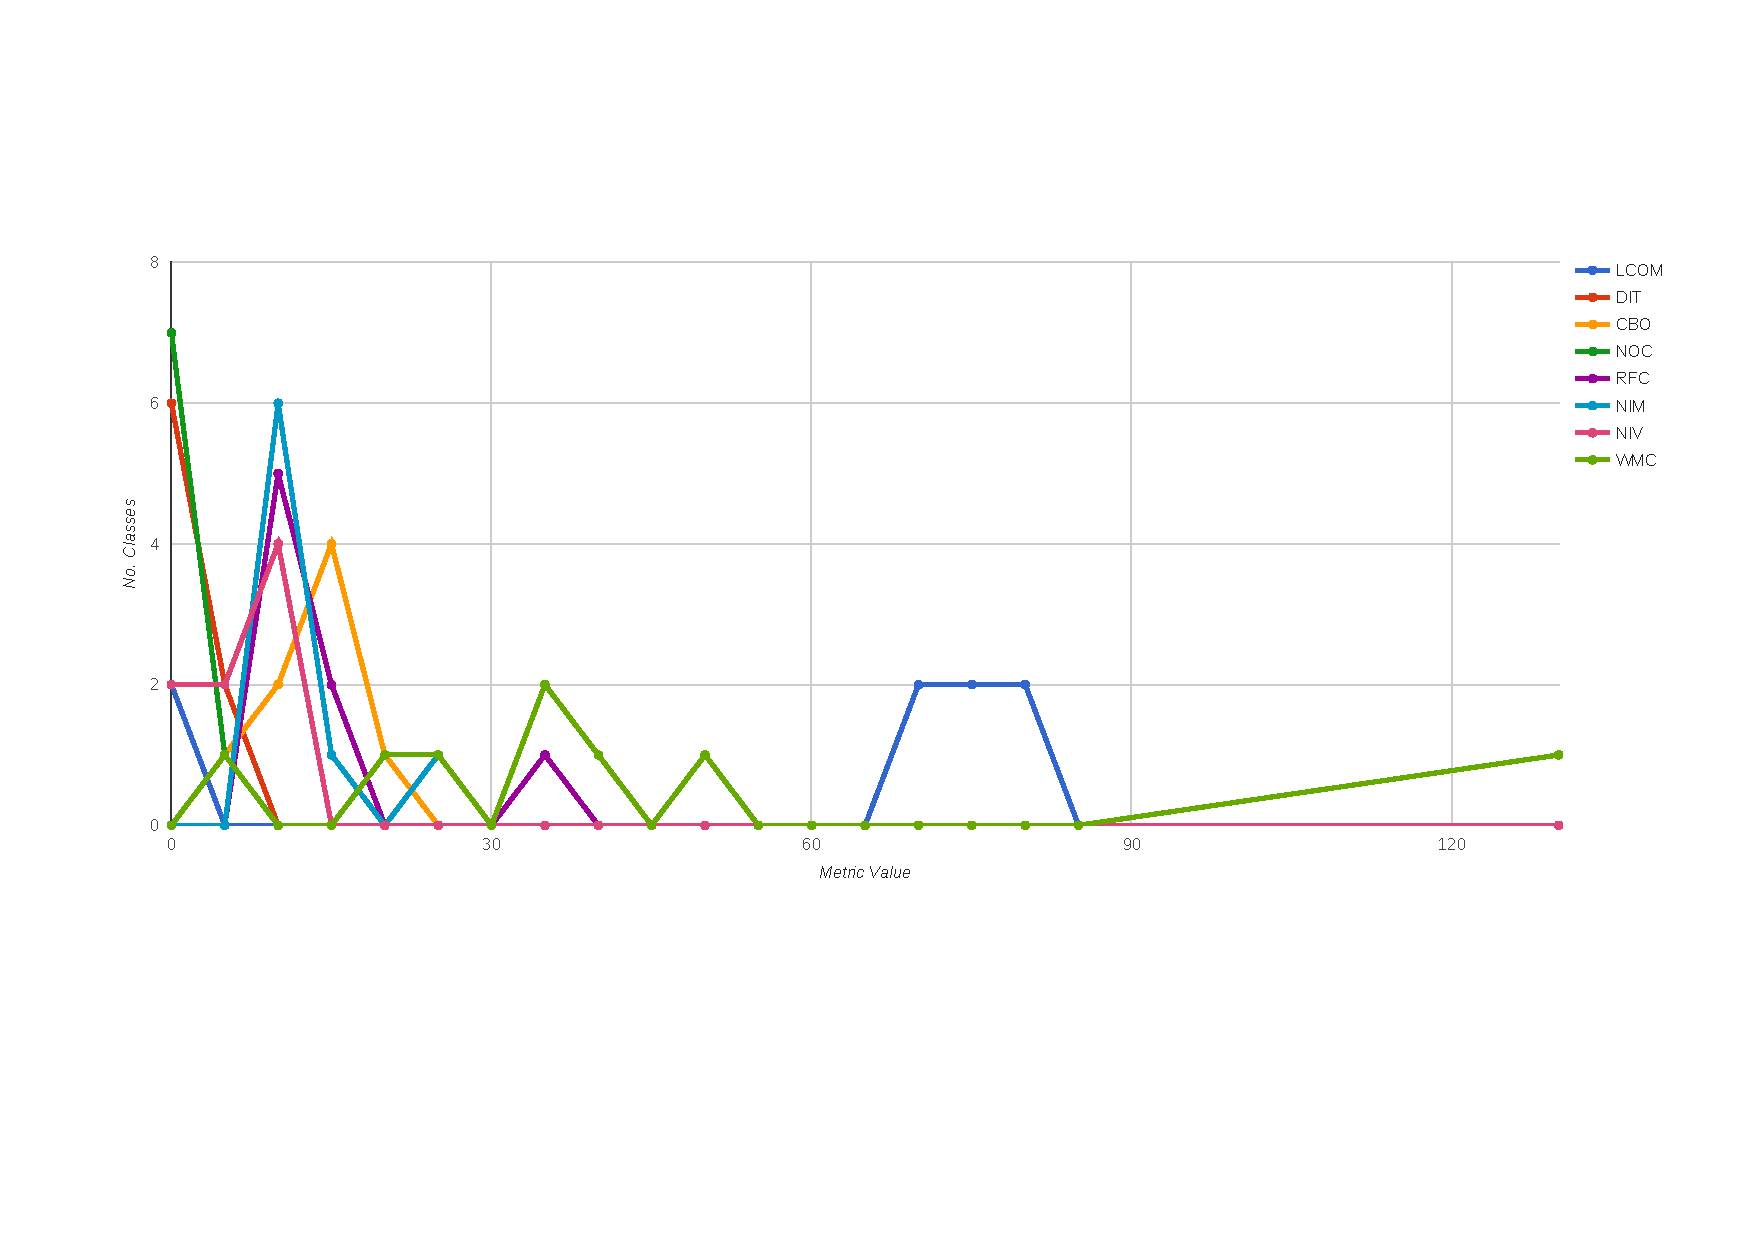
\includegraphics[width=\textwidth]{images/pdf/network.pdf}
	\caption{Frequency distribution of OO-metrics in Component N}
	\label{fig:netgraph}
	\end{figure}
\end{landscape}



\subsubsection{Component P}
The descriptive statistics calculated for Component P are presented in Table \ref{tab:oometrics-proc}. The frequency distribution of the metrics are presented in Figure \ref{fig:procgraph}. We identified 12 files in Component P, consisting of 12 files, 722 lines of code, and 8 classes.

LCOM values in Component P ranges from 0 to 81. A median value shows the level of cohesiveness in the system. In this context, the median value shows that more than half of the classes have large LCOM values, implying that these classes are improperly designed and should be split up to make them more cohesive. We identified three classes with values of LCOM larger than 70. The DIT results range from 0 to 1, implying that most classes have flat inheritance hierarchies. There are only 2 classes having a DIT value of 1. Despite the fact that 6 of the classes have DIT metric of 0, they alone may not tell us if classes are part of an inheritance tree or if they are root classes. By examining the NOC results, we see that only one class has a NOC value of 1. Six classes have both NOC and DIT values of zero, indicating that they are not part of an inheritance hierarchy. CBO values ranges from 0 to 12, with a mean and median of 5.5. WMC values range from 1 to 47. 


\begin{table}[]
\resizebox{\textwidth}{!}{
\centering
\caption{OO-metrics and descriptive statistics for Component P}
\label{tab:oometrics-proc}
\begin{tabular}{|l|l|l|l|l|l|l|l|}
\hline
\textbf{Metric} & \textbf{Min} & \textbf{Max} & \textbf{Median} & \textbf{Sample Mean} & \textbf{Standard Deviation} & \textbf{Kurtosis} & \textbf{Skewness} \\ \hline
LCOM            & 0            & 81           & 63              & 57.25                & 25.409     & 4.625  & -1.987                   \\ \hline
DIT             & 0            & 1            & 0               & 0.25                 & 0.463    & 0 & 1.440                     \\ \hline
CBO             & 0            & 13           & 6             & 6                  & 4.472        & -0.645  & 0.255                 \\ \hline
NOC             & 0            & 1            & 0               & 0.125                & 0.353     & 8  & 2.828                    \\ \hline
RFC             & 2            & 14           & 6.5             & 7.375                  & 3.502     & 1.523  & 0.647                    \\ \hline
NIM             & 2            & 13           & 6.5             & 6.875                    & 3.044   & 2.986  & 0.765                      \\ \hline
NIV             & 0            & 6            & 3.5             & 3.125                & 2.031     & -0.886  & -0.223                    \\ \hline
WMC            & 1            & 47           & 8               & 15.75                & 15.809     & -1.037  & 1.350                   \\ \hline
\end{tabular}}
\end{table}



\begin{landscape}
\setlength\LTleft{-.5in}
	\begin{figure}
	\centering
	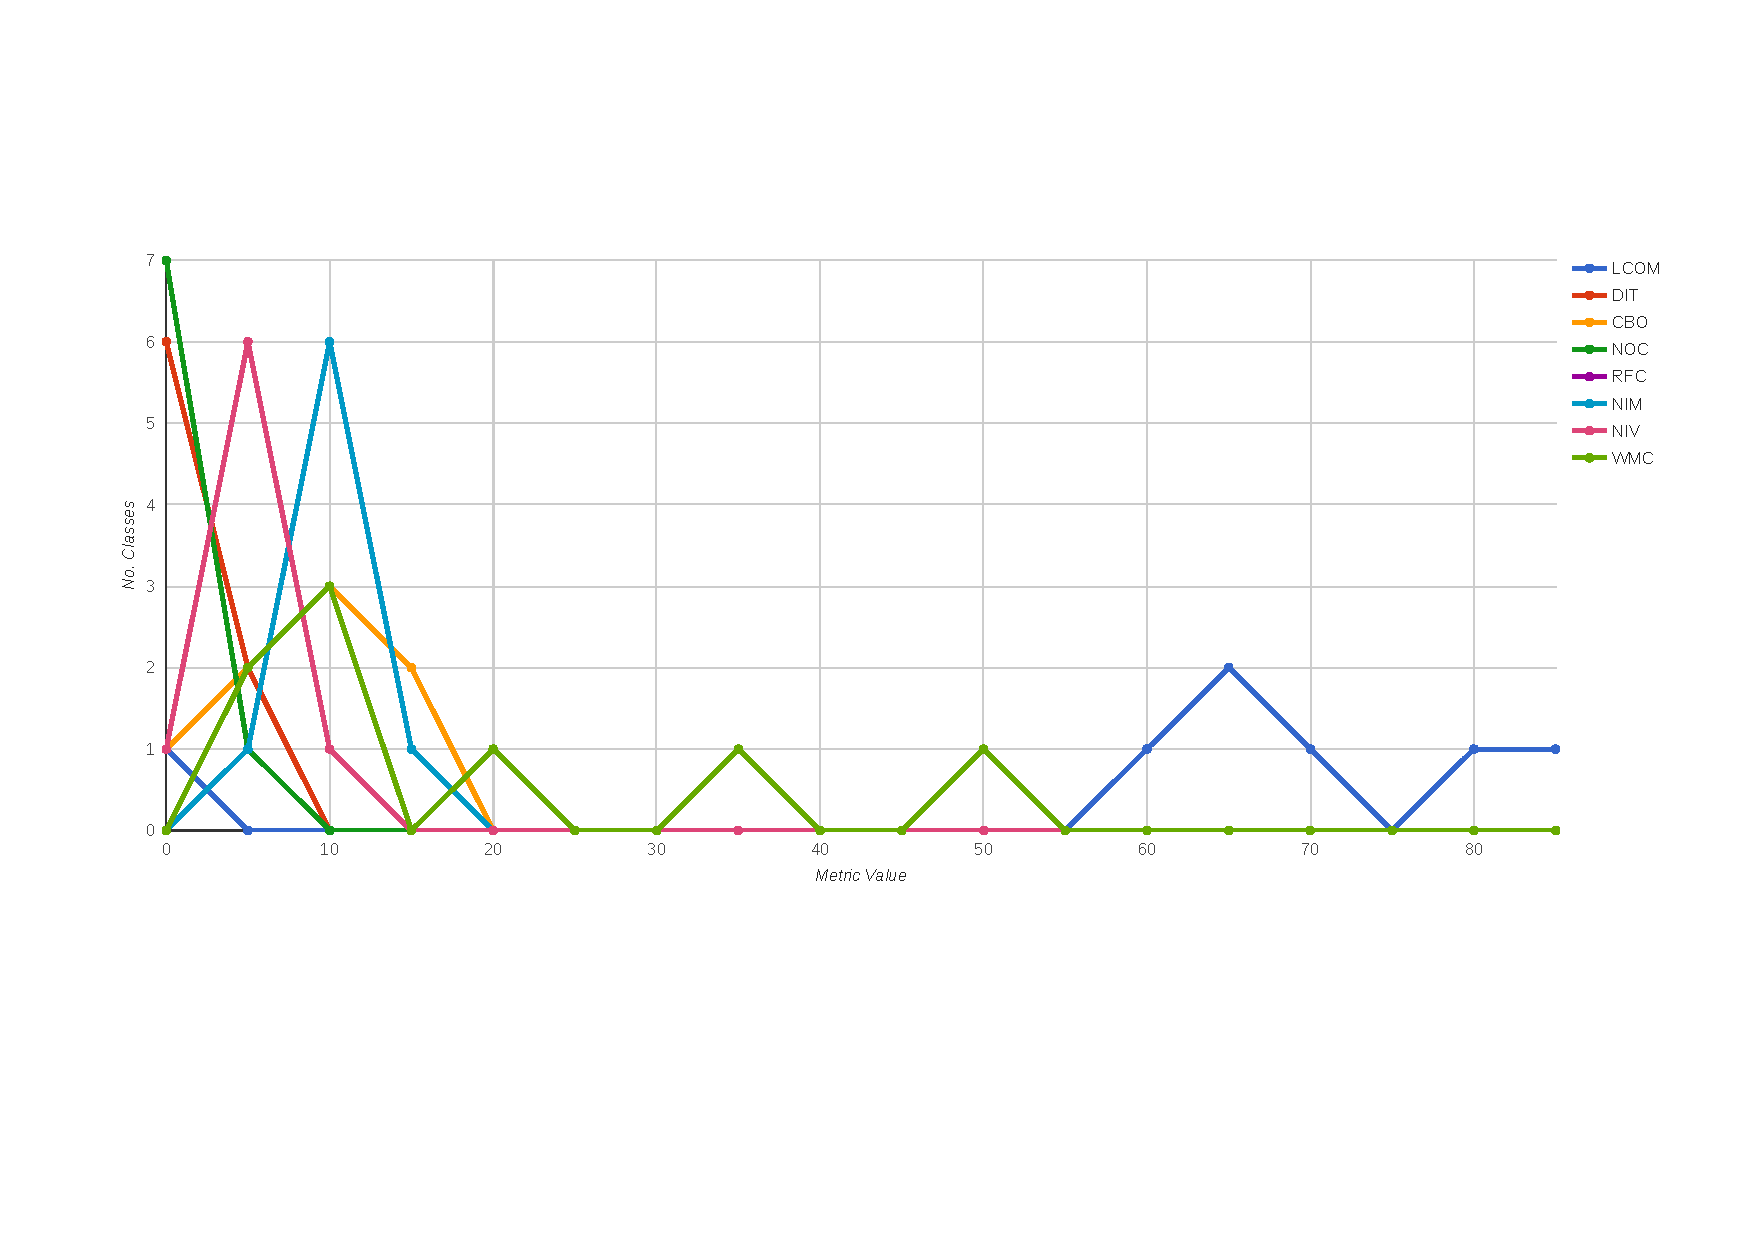
\includegraphics[width=\textwidth]{images/pdf/process.pdf}
	\caption{Frequency distribution of OO-metrics in Component P}
	\label{fig:procgraph}
	\end{figure}
\end{landscape}



\subsubsection{Component S}
Table \ref{tab:oometrics-sys} presents the descriptive statistics for Component S. Component S contains 4 files, which consists of 223 lines of code and 2 classes. The LCOM values show that there are possibilities to improve the design of this component by splitting up methods that does not share fields with each other to separate classes. Moreover, the results point out that none of the classes has any subclasses. However, the results reveal that one of the classes inherits methods and variables from a superclass. Moreover, WMC metric values indicate that the classes have less complexity and greater polymorphism.

\begin{table}[]
\resizebox{\textwidth}{!}{
\centering
\caption{OO-metrics and descriptive statistics for Component S}
\label{tab:oometrics-sys}
\begin{tabular}{|l|l|l|l|l|l|l|l|}
\hline
\textbf{Metric} & \textbf{Min} & \textbf{Max} & \textbf{Median} & \textbf{Sample Mean} & \textbf{Standard Deviation} & \textbf{Kurtosis} & \textbf{Skewness} \\ \hline
LCOM            & 33           & 50           & 41.5            & 41.5                 & 12.021   & N/A & N/A                     \\ \hline
DIT             & 0            & 1            & 0.5             & 0.5                  & 0.707     & N/A  & N/A                    \\ \hline
CBO             & 3            & 7            & 5             & 5                  & 2.829         & N/A  & N/A                \\ \hline
NOC             & 0            & 0            & 0               & 0                    & 0         & N/A  & N/A                    \\ \hline
RFC             & 6            & 9            & 7.5             & 7.5                  & 2.121          &N/A  & N/A               \\ \hline
NOM             & 6            & 9            & 7.5             & 7.5                  & 2.121          & N/A  & N/A               \\ \hline
NIM             & 6            & 9            & 7.5             & 7.5                  & 2.121        & N/A  & N/A                 \\ \hline
NIV             & 1            & 1            & 1               & 1                    & 0     & N/A  & N/A                        \\ \hline
WMC            & 6           & 19            & 12.5            & 12.5                 & 9.192        & N/A  &  N/A                   \\ \hline
\end{tabular}}
\end{table}

 

\subsubsection{Component W}
Component W contains only one file. This file consists of 69 lines of code. This component has one class. The class have a LCOM value of 58, indicating that some instance variables are not shared across the member functions. Moreover, DIT and NOC values of 0 indicates that this class does not inherit from a superclass, or has any subclasses. The results reports a CBO value of 4, implying that this class is not tightly coupled with other objects. There are only 2 instance variables in this class, and 6 methods, in which all are instance methods. WMC value of this class is set to 8.




% Our results show that (whats good and wrong with these metrics, what can be done). 


% HVA SLAGS METRIKKER ER INTERESSANT, GÅ DYPERE INN PÅ DEM. F.EKS METHODS IN CLASS, HVA SIER DET OSS

% TOO MANY LINES OF CODE? CHECK SINGLE RESPONSBILITY PRINCIPLE, it states that every class or module should have responsbility for a single part of the funcitnaility provided by the software.'





\section{Identifying Code Smells using Automatic Static Analysis Tools}
\label{sub:code_smell_detection}
Code smells are used to find problematic classes. As we explained in Chapter \ref{chap:sota}, one of the ways to identify DD is to look at the number of code smell in the source code. Code smells are an indicator of software design flaws in OO-systems that can decrease software maintainability which may lead to issues in further evolution of the system\cite{olbrich2009evolution}. The analysis of code smells in the system is based on ASA tools. We investigated each tool that we could use in this project, and evaluated the smells they are able to detect. Table \ref{tab:identifiedCodeSmell} describes the number of code smells that were identified using automatic static analysis tools.

\begin{table}[ht!]
\centering
\caption{Number of Code Smells detected}
\label{tab:identifiedCodeSmell}
\begin{tabular}{|l|p{3cm}|}
\hline
\textbf{Code Smell}                           & \textbf{Detected}    \\ \hline
Long Method                                   & 10          \\ \hline
% Large Class                                   & 8          \\ \hline
Long Parameter List                           & 15          \\ \hline
Duplicated Code                               & Approximately 5\% of the source code.  \\ \hline
Speculative Generality                        & 1153      \\ \hline
Dead Code 									  & 151 \\ \hline
\end{tabular}
\end{table}

\subsubsection{Duplicated Code}
\textit{Duplicated Code} is found by looking for pieces of code that appears at multiple places in the source code, both internally in a file or in another file. A piece of code is considered duplicated if the piece of code contains at least 10 lines of code and occurs at multiple places in the source code. Table \ref{tab:identifiedCodeSmell} shows the number of duplicated code found by \textit{SonarQube}, expressed as a percentage value. The results show that roughly 5\% of the source code contains duplicated code including the test files. This corresponds to approximately 4395 lines of code, affecting 39 files across the system. We identified that roughly 54\% of the duplicated code is located in Component A. The other duplicated lines are spread across Component B, N, P, C, D, L, Ex, S, and G. Table \ref{tab:duplicatedLines} summarizes duplicated lines in the different components. The first column contains the name of the components, while the second column summarizes number of files affected by duplicated code and the number of duplicated lines among these files.

\begin{table}[ht!]
\centering
\caption{Duplicated Code in Project "Firmus"}
\label{tab:duplicatedLines}
\begin{tabular}{|l|l|}
\hline
\textbf{Component}			& \textbf{Information} \\ \hline
Component A 				& 12 files, 2400 LOC \\ \hline
Component B 				& 6 files, 366 LOC \\ \hline
Component C 				& 3 files, 284 LOC \\ \hline
Component D 				& 2 files, 80 LOC \\ \hline
Component Ex 				& 4 files, 305 LOC \\ \hline
Component G 				& 4 files, 311 LOC \\ \hline
Component L 				& 1 file, 30 LOC \\ \hline
Component N 				& 3 files, 301 LOC \\ \hline
Component P 				& 2 files, 124 LOC \\ \hline
Component S 				& 2 files, 194 LOC \\ \hline
\end{tabular}
\end{table}


\subsubsection{Long Method}
\textit{Understand for C++} considers a \textit{Long Method} as code smell if lines of code in method exceeds 200 lines. We identified 10 long methods, spread across six different files. 7 of 10 long methods are located in the test files. 

\subsubsection{Long Parameter List}
\textit{Long Parameter List} code smell is detected by comparing the total number of parameters in a method against a fixed threshold. The maximum number of parameters allowed in a method using \textit{CppDepend} is set to 5. This means that 6 or more parameters in a method are considered as code smell. The results from CppDepend report 15 hits of \textit{Long Parameter List} code smell, where 3 hits are considered as critical. A \textit{Long Parameter List} is considered as critical when total of parameters in a method is higher than 8. The largest number of parameters in a method we identified was 12. These results were verified manually by examining the class diagrams for the corresponding methods.

\subsubsection{Speculative Generality}
\textit{Speculative Generality} is detected by detecting unused classes, methods, fields, or parameters. Table \ref{tab:speculativeGenerality} summarizes \textit{Speculative Generality} code smell that were identified through a code analysis using \textit{Understand for C++}. The results are divided into the categories unused methods, unused local variables, and unused static globals. 

\begin{table}[ht!]
\centering
\caption{Speculative Generality in Project "Firmus"}
\label{tab:speculativeGenerality}
\begin{tabular}{|l|l|}
\hline
\textbf{Category}		& 	\textbf{Hits} \\ \hline
Unused Methods 			&	794  \\ \hline
Unused Local Variables 	& 	346	 \\ \hline
Unused Static Globals 	& 	13	 \\ \hline
\end{tabular}
\end{table}

%\subsubsection{Shotgun Surgery}
%The results shows that X classes are infected with the Shotgun Surgery code smell. 

%CBO and LCOM can be useful to detect God Classes with support of LOC and WMC. (article: on the effectiveness of concern metrics to detect code smells: an empirical study)

%A class with large values of WMC and RFC indicates many possible re since the class may have a large number of methods that can be executed. These values along with LCOM can be used to measure God Class code smell. By identiying 

%5 files
%AL: LogicsEngine
%Autrologic: LogicsUnitDetectionZone
%Autrologic: Logicsunit
%AL: LogicsUnitFad (kasnkje)
%BLC: AclibTranslator

\subsubsection{Dead Code}
Fowler and Beck\cite{1999:RID:311424} do not classify \textit{Dead Code} as code smell. However, \textit{Dead Code} should be classified as a code smell, as it is a quite common problem as it hinders code comprehension and makes the current program structure less obvious\cite{mantyla2003taxonomy}. We examined three types of \textit{Dead Code} code smell in Project "Firmus": "Commented Out" Code, Unreachable Code, and Unnecessary Includes in Header Files. In total, we found 151 hits of \textit{Dead Code} code smell, which we have summarized in Table \ref{tab:deadCode}.

\begin{table}[ht!]
\centering
\caption{Dead Code in Project "Firmus"}
\label{tab:deadCode}
\begin{tabular}{|l|l|}
\hline
\textbf{Category}		& 	\textbf{Hits} \\ \hline
"Commented Out" Code 			&	67  \\ \hline
Unreachable Code 	& 	10	 \\ \hline
Unnecessary Includes in Header Files 	& 	74	 \\ \hline
\end{tabular}
\end{table}

% ANtiåpattern, move down to metrics, point out that possible god classes may be antipatterns.



%How did we study the different code smells, the apporach and the results.
%The results from Table XX

%As we see, there are many code smells detected. We take a closer look at some of the classes; presented in UML diagrams here:




































